\appendix

\section {X-ray Event Selection}\label{app:selection}
The X-ray events are selected using
the integrated charge, waveform amplitude and
timing, calculated over the scanned 
and background regions.
The selection criteria and the distribution of variables are given below. 
\begin{enumerate}
\item Time Waveform Peak: $-700 < T_{peak} <-500$ ns
\item Sum charge: $\Sigma Q<$1.5 pC
\item Mean background charge: $\bar{Q}_{bkg}<$0.2 pC, with either 4 or 8 background channels
\item Waveform Amplitude: $A_i>$50 mV. 
\end{enumerate}
\begin{figure}[h]
    \centering
    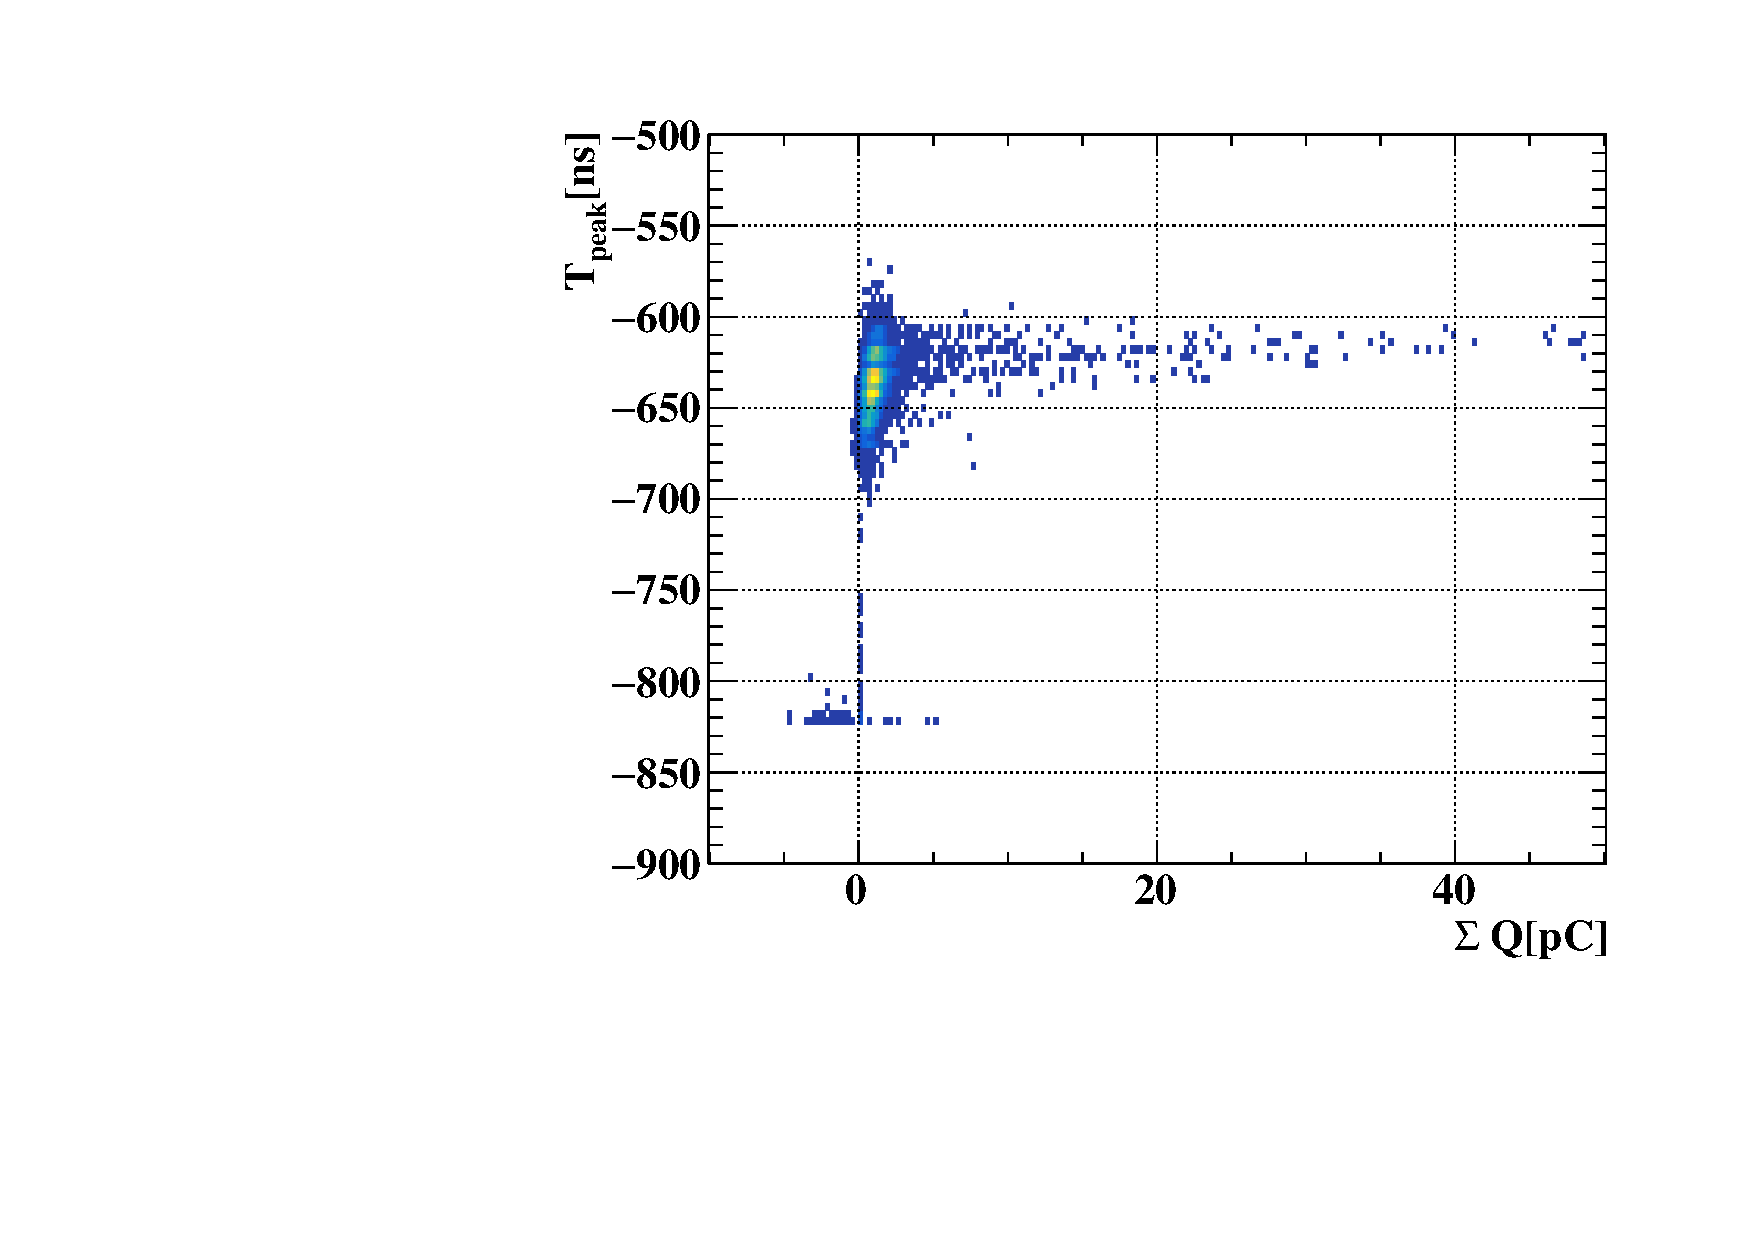
\includegraphics[width=.4\linewidth]{plots/2018/Sel1}
    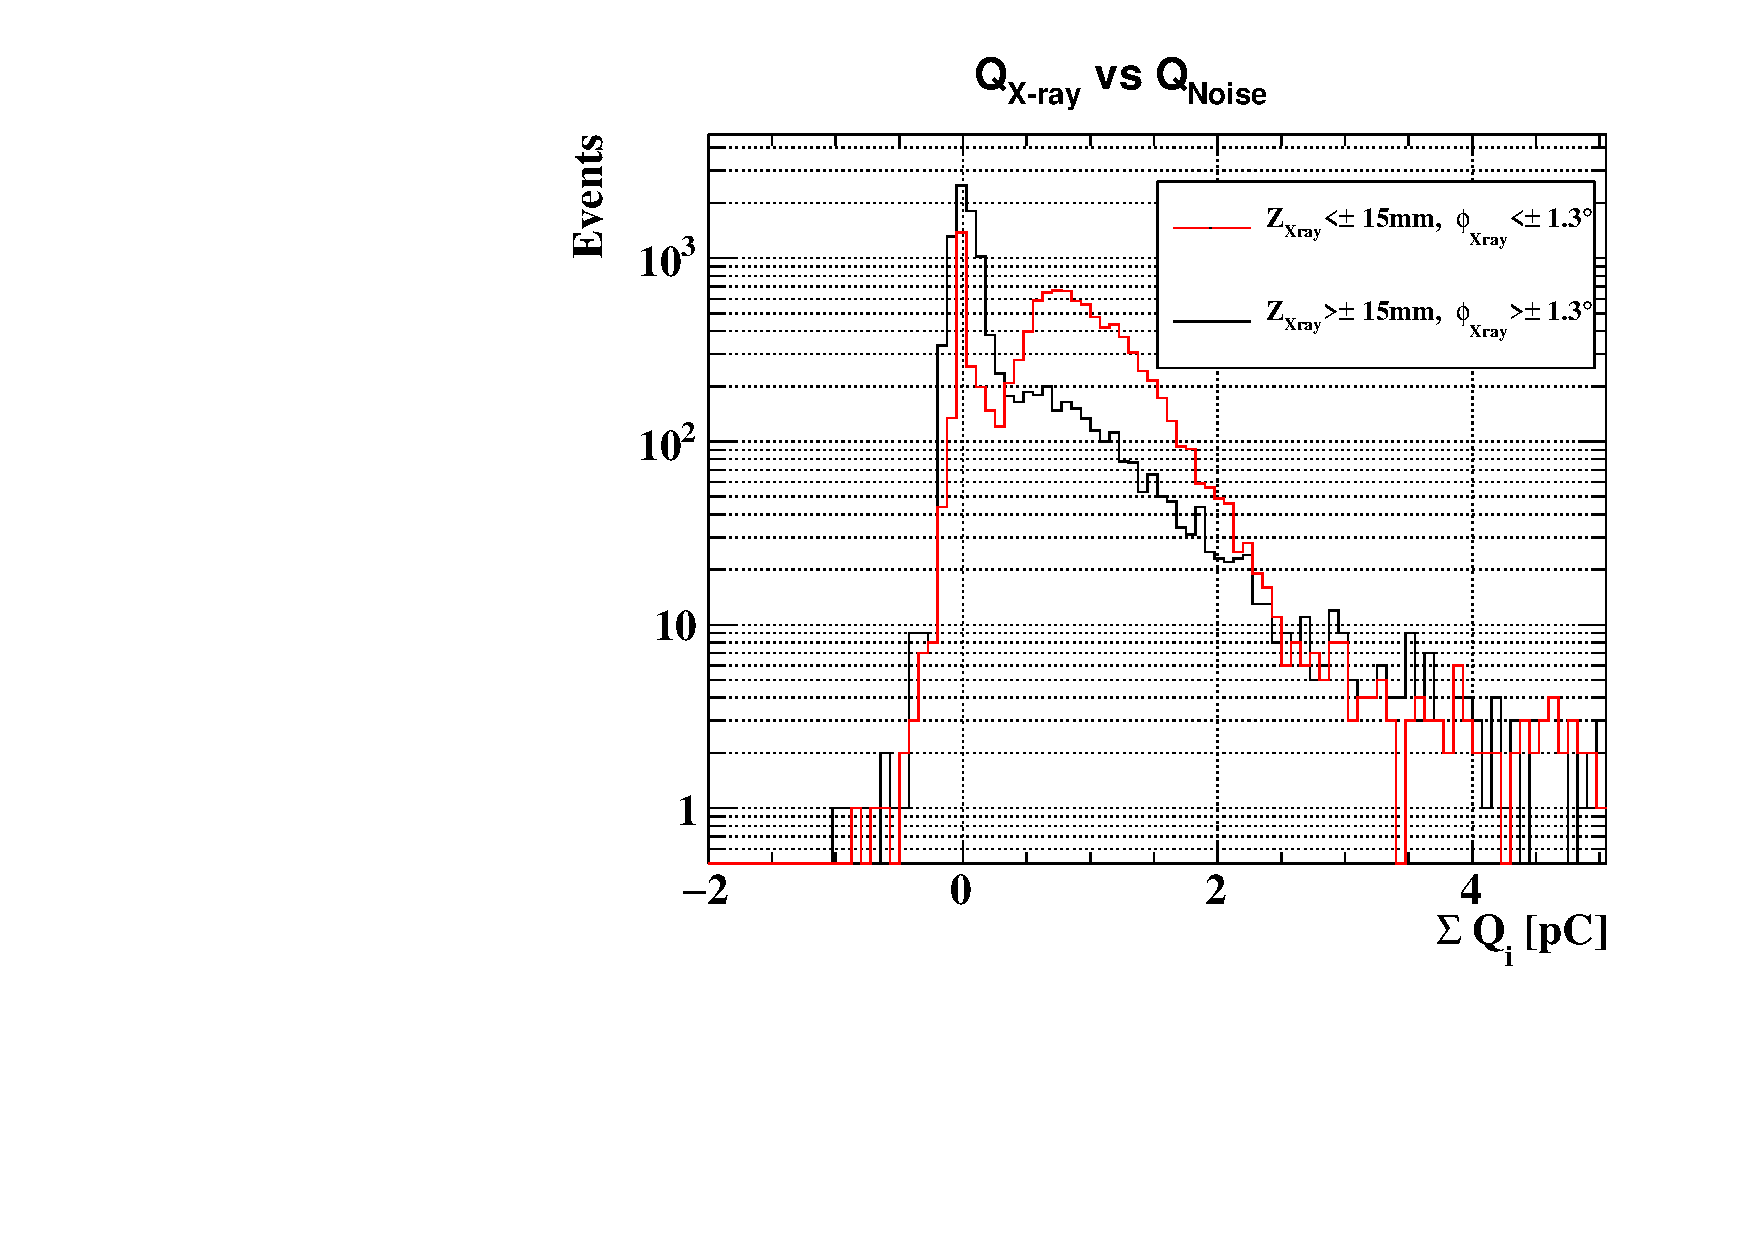
\includegraphics[width=.4\linewidth]{plots/2018/Sel2}\\
    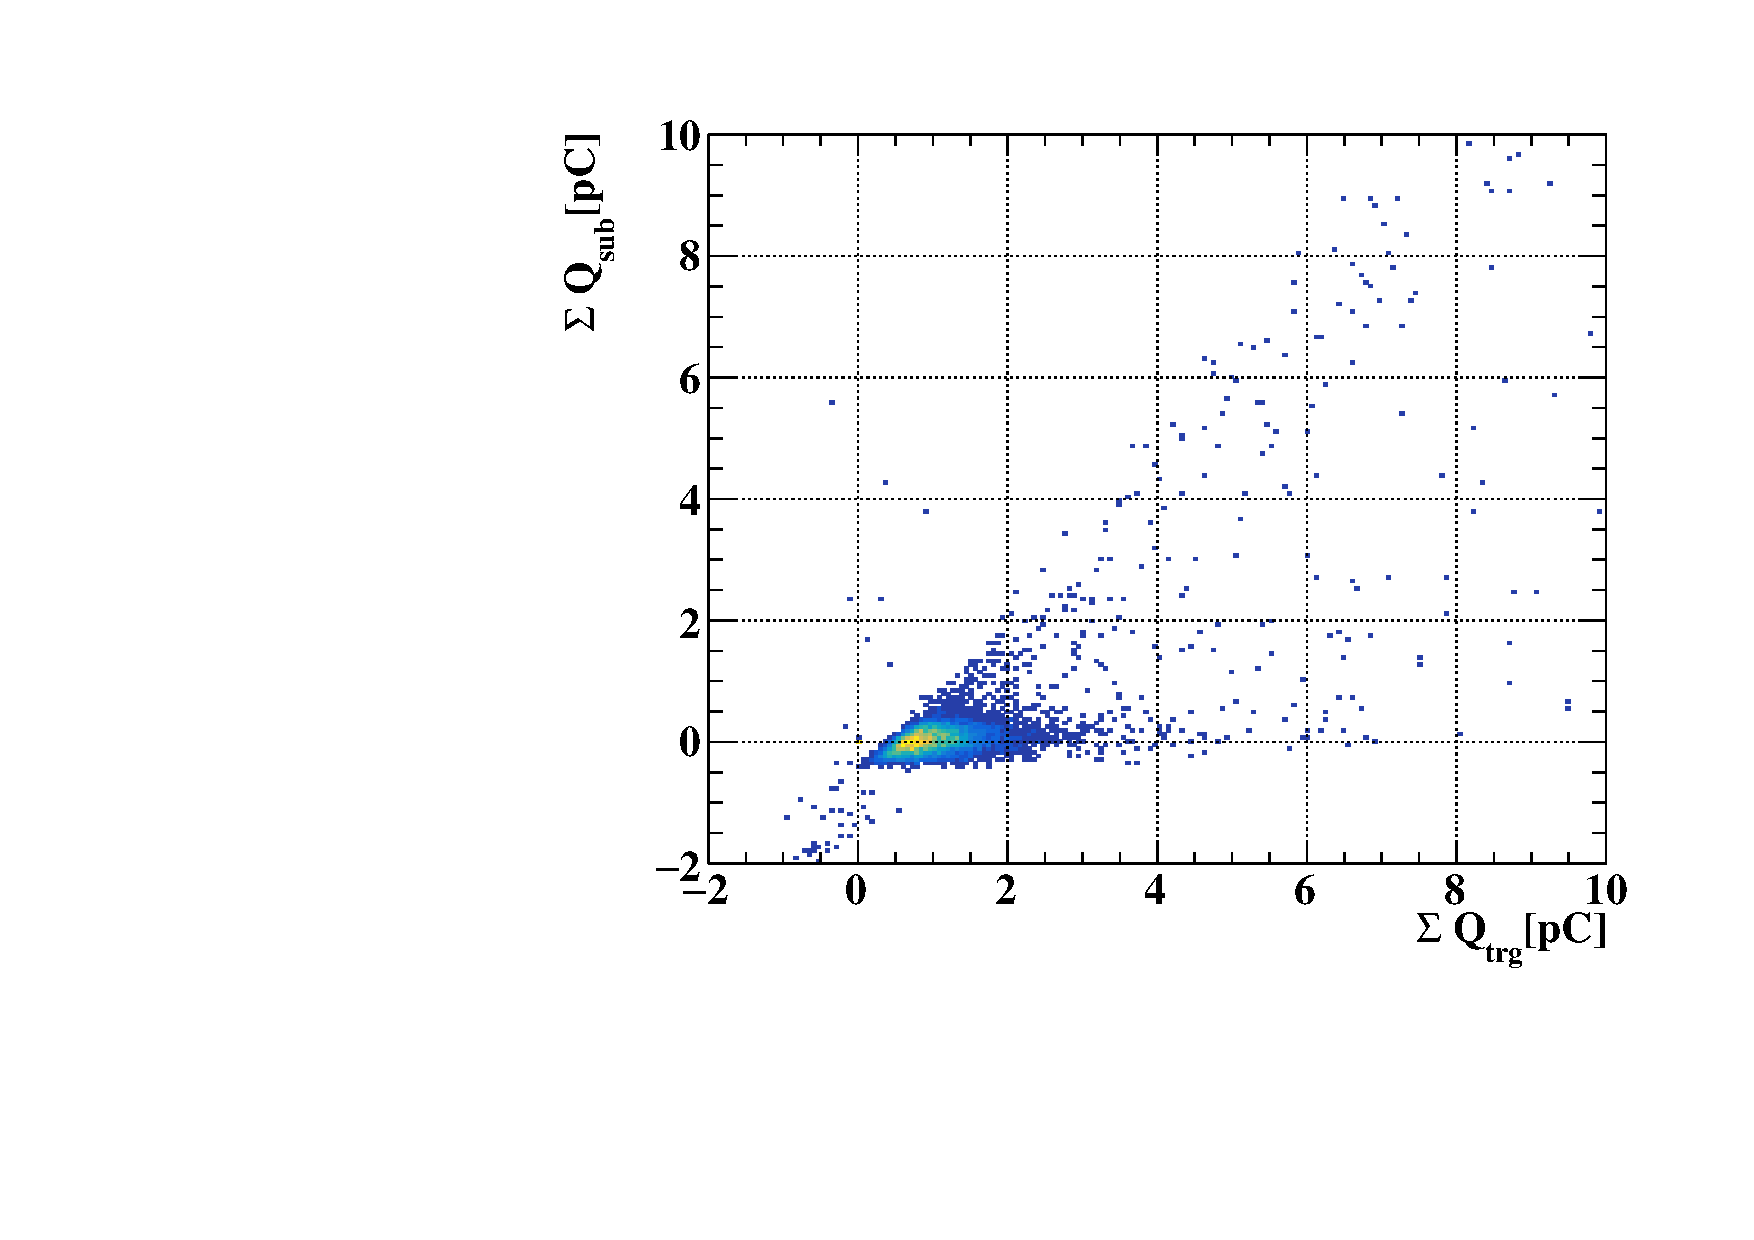
\includegraphics[width=.4\linewidth]{plots/2018/Sel3}
    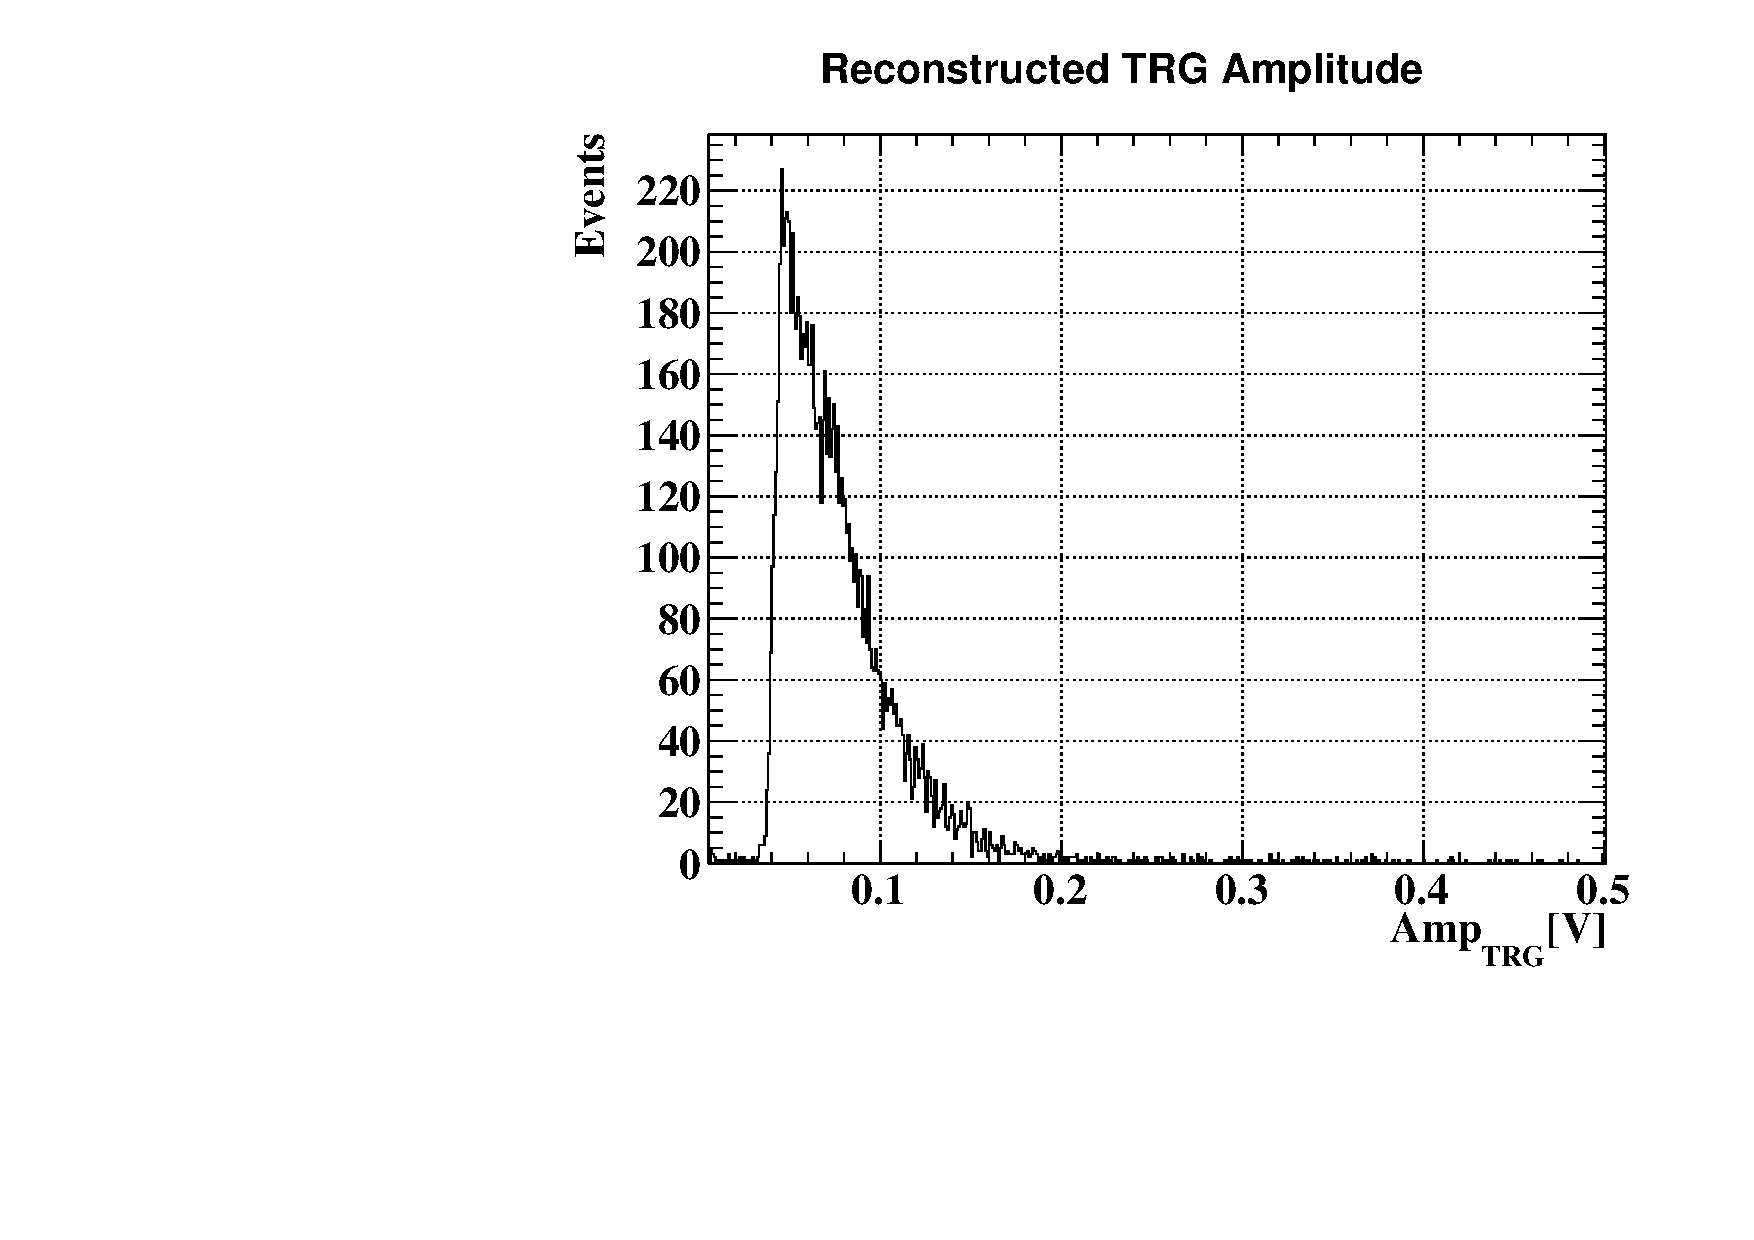
\includegraphics[width=.4\linewidth]{plots/2018/Sel4}
  \label{fig:selectionvariables}
  \caption{Variables used for X-ray event selection.}
\end{figure}

The left and right halves of the photodetector along the $\hat{z}$ direction
show different response to the X-ray signal (Sec.\ref{sec:qegain}).  In fig.
\ref{fig:mppcleftright} the mean charge and waveform amplitude are calculated
from the entire dataset, showing disparity in both observables; 
greater in charge (10\%) than in waveform amplitude(3\%). 
As a result, the reconstructed positions using the two criteria are 
displaced with respect to each other. Since the polarity of left-right
response changes about the center line (Z = 0 mm), the direction of
displacement also changes correspondingly (fig. \ref{fig:chargevswfamp}).

\begin{figure}[h]
    \centering
    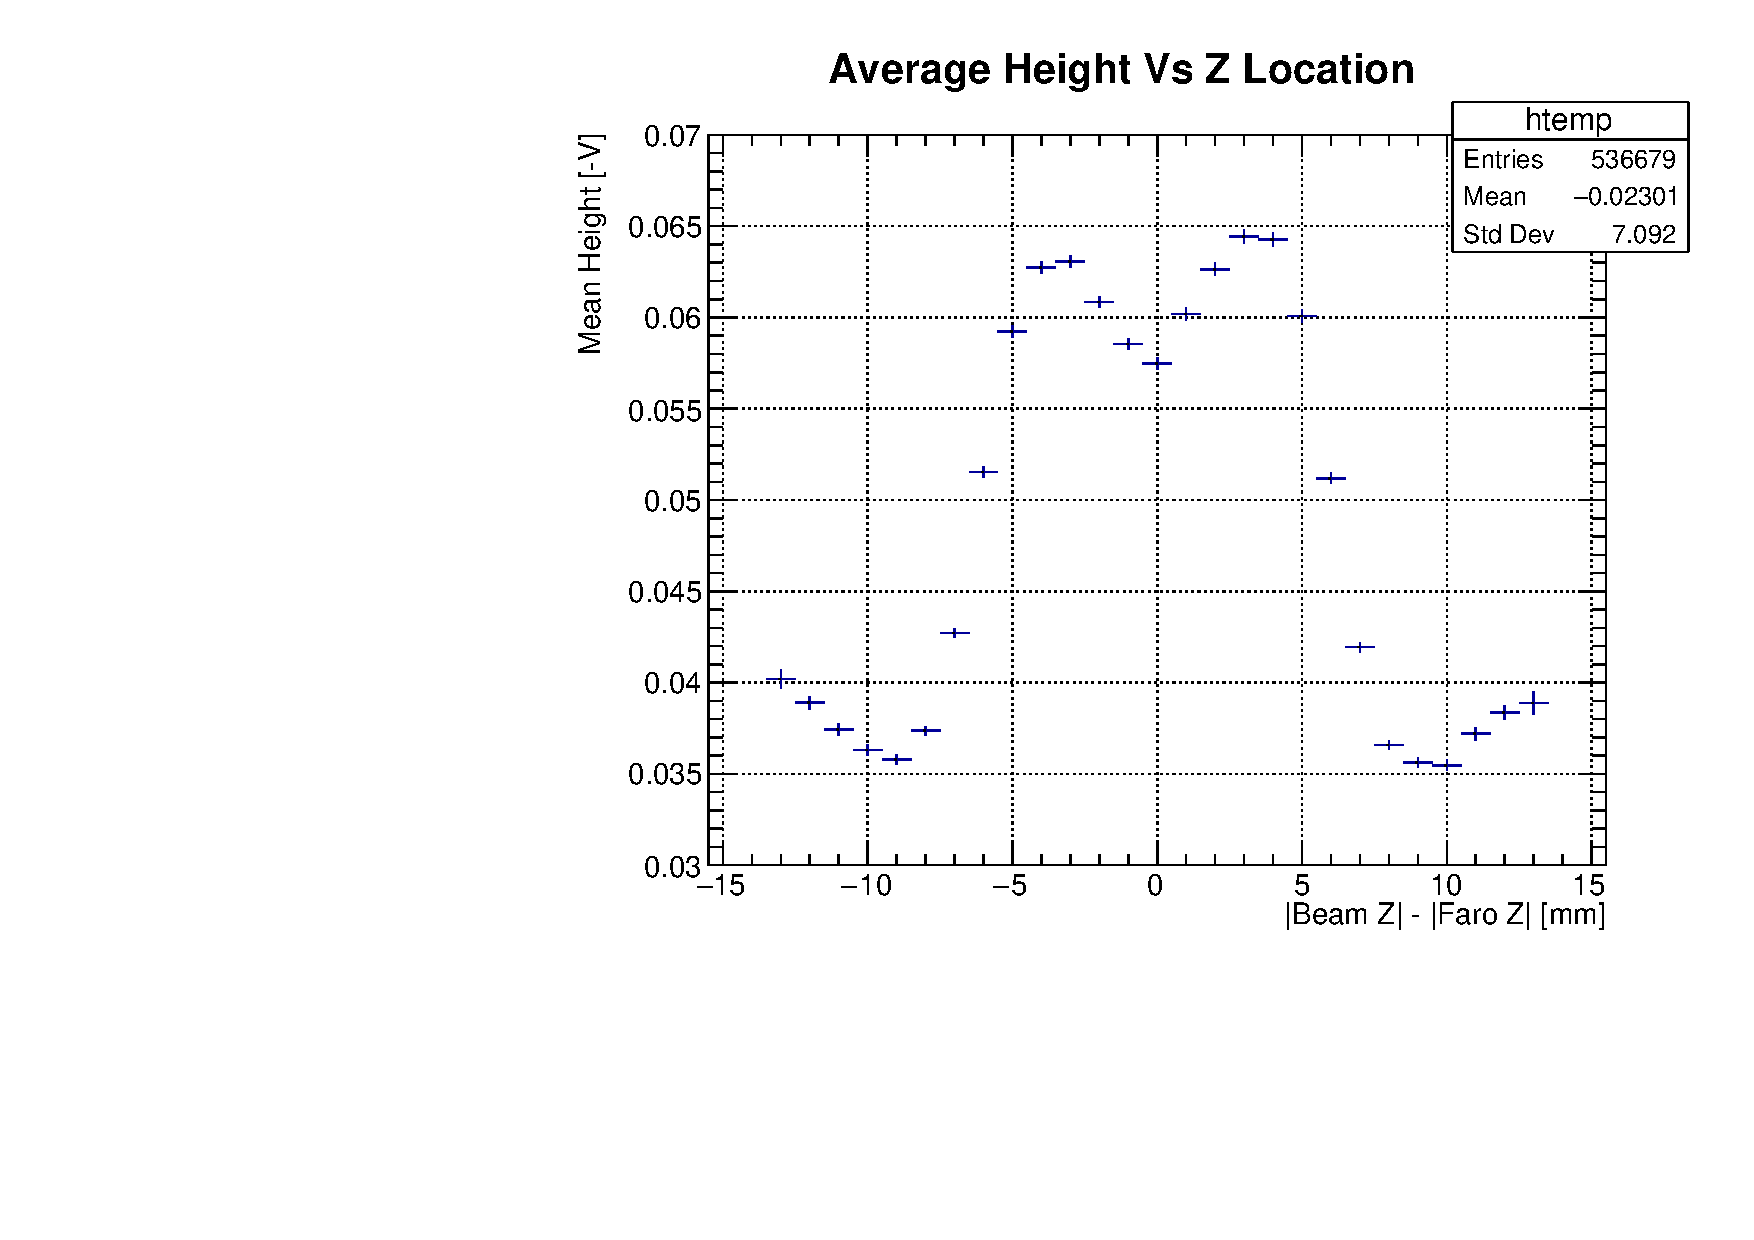
\includegraphics[width=.4\linewidth]{plots/2018/HeightvsZ2}
    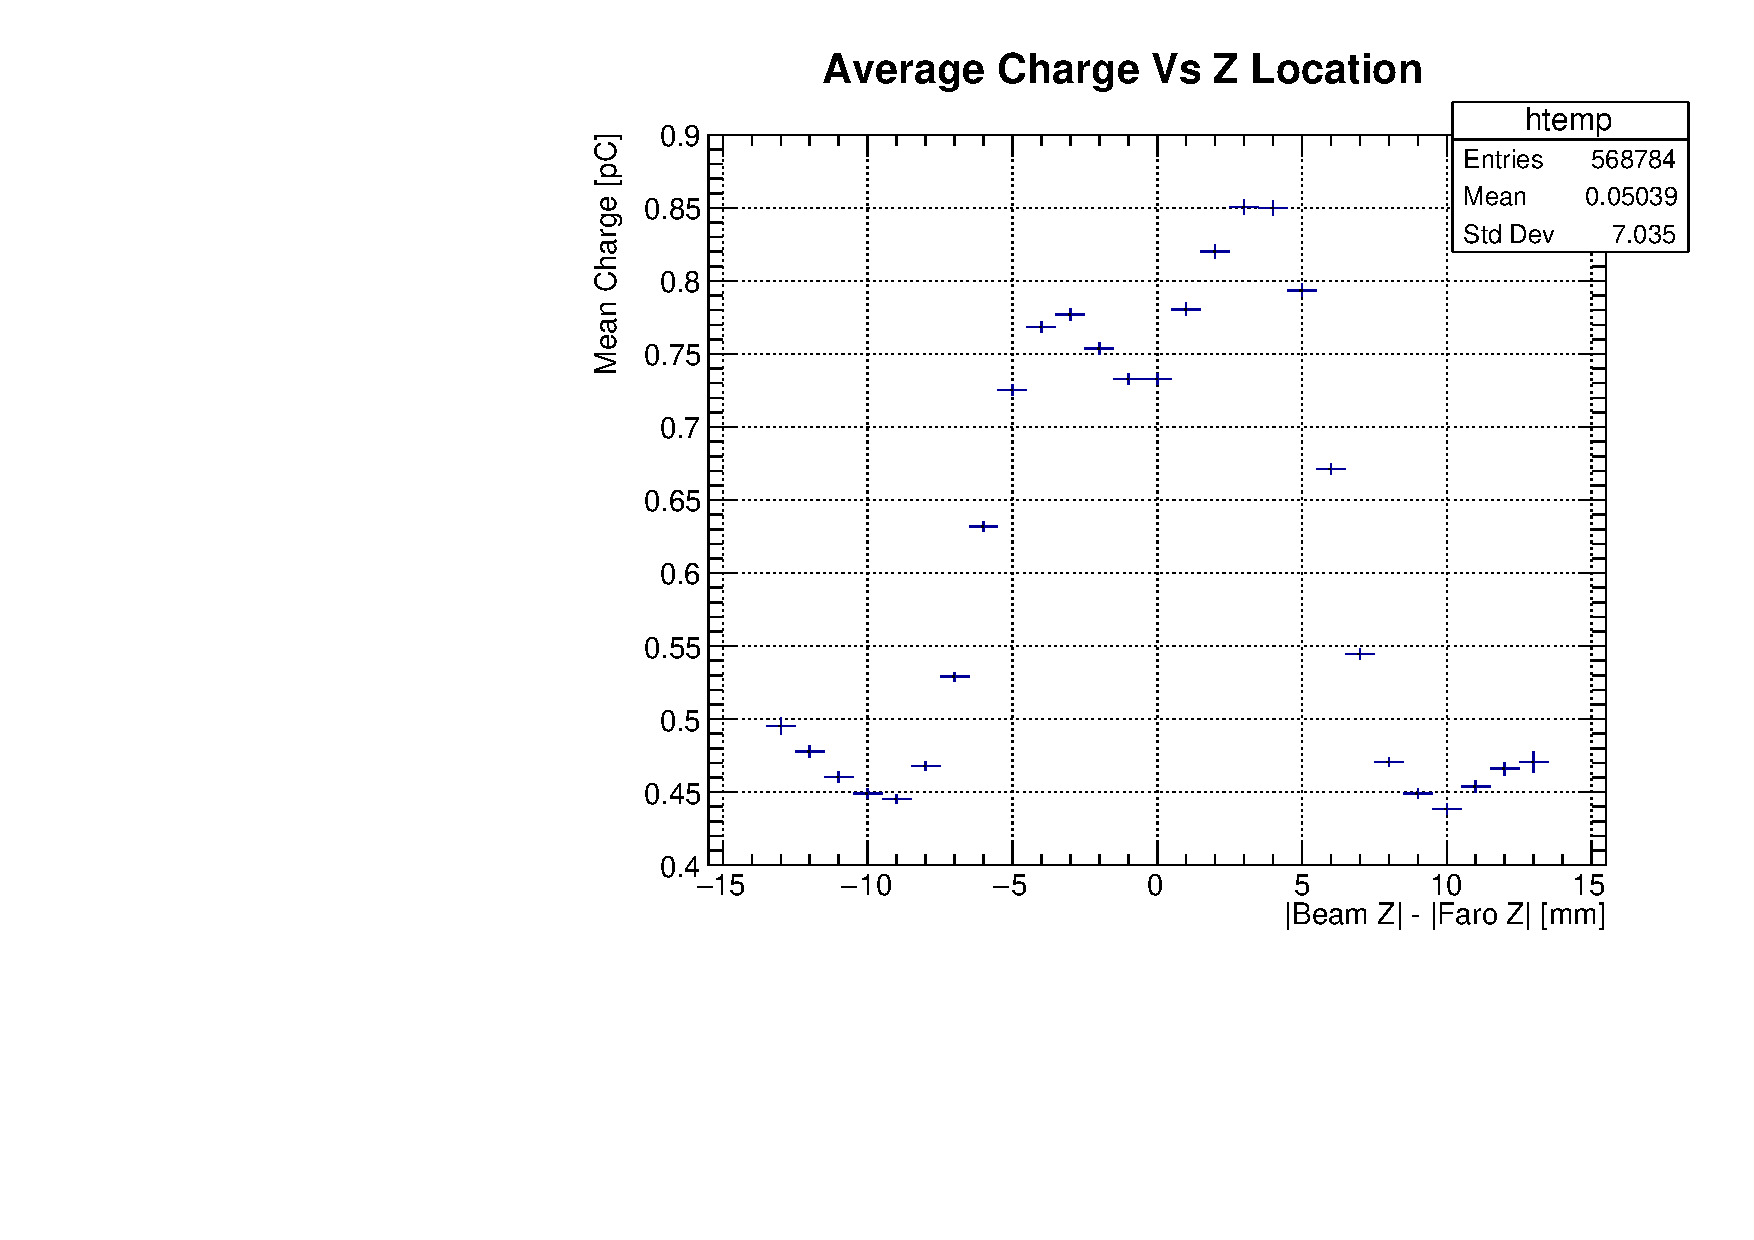
\includegraphics[width=.4\linewidth]{plots/2018/ChargevsZ2}
  \caption{Mean waveform amplitude (left) and charge (left) as a function of X-ray Z coordinate centered
    at nominal photodetector center. Only downstream photodetectors ($Z>0$ mm) are included in the plot.}
  \label{fig:mppcleftright}
\end{figure}

\begin{figure}[h]
    \centering
    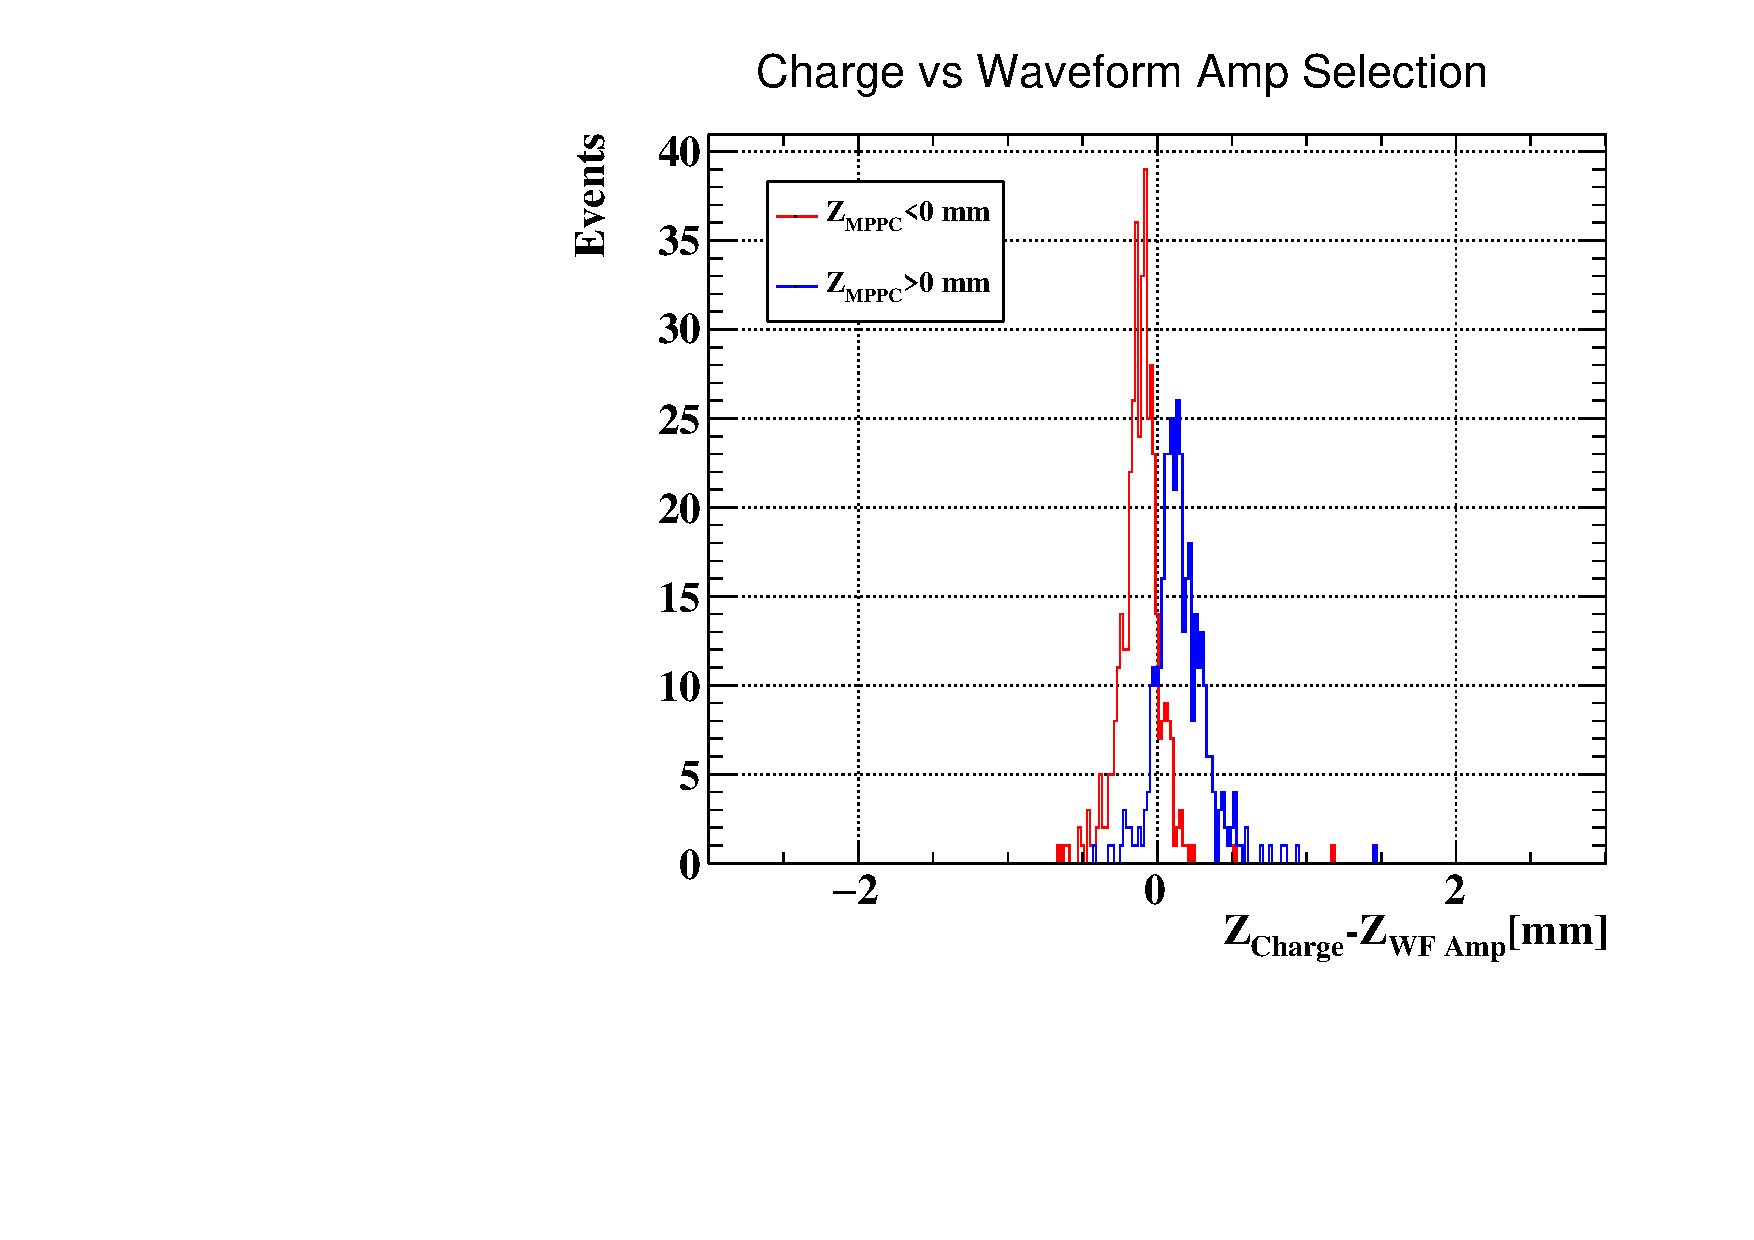
\includegraphics[width=.4\linewidth]{plots/2018/chargevswfampZ}
  \caption{Difference in the reconstructed Z position of the photodetectors 
   due to selection based on charge and waveform amplitude.}
  \label{fig:chargevswfamp}
\end{figure}



\section{Fit Values and Errors}
Fitted parameter values and parameter errors for the primary fit 
function. 

\begin{enumerate}
    \item Z Position Fit Error $<$ 0.3 mm
    \item $\phi$ Position Fit Error $<$ 0.03 deg
    \item Reduced $\chi ^{2} \; <$ 100
\end{enumerate}


\begin{figure}[h]
    \centering
    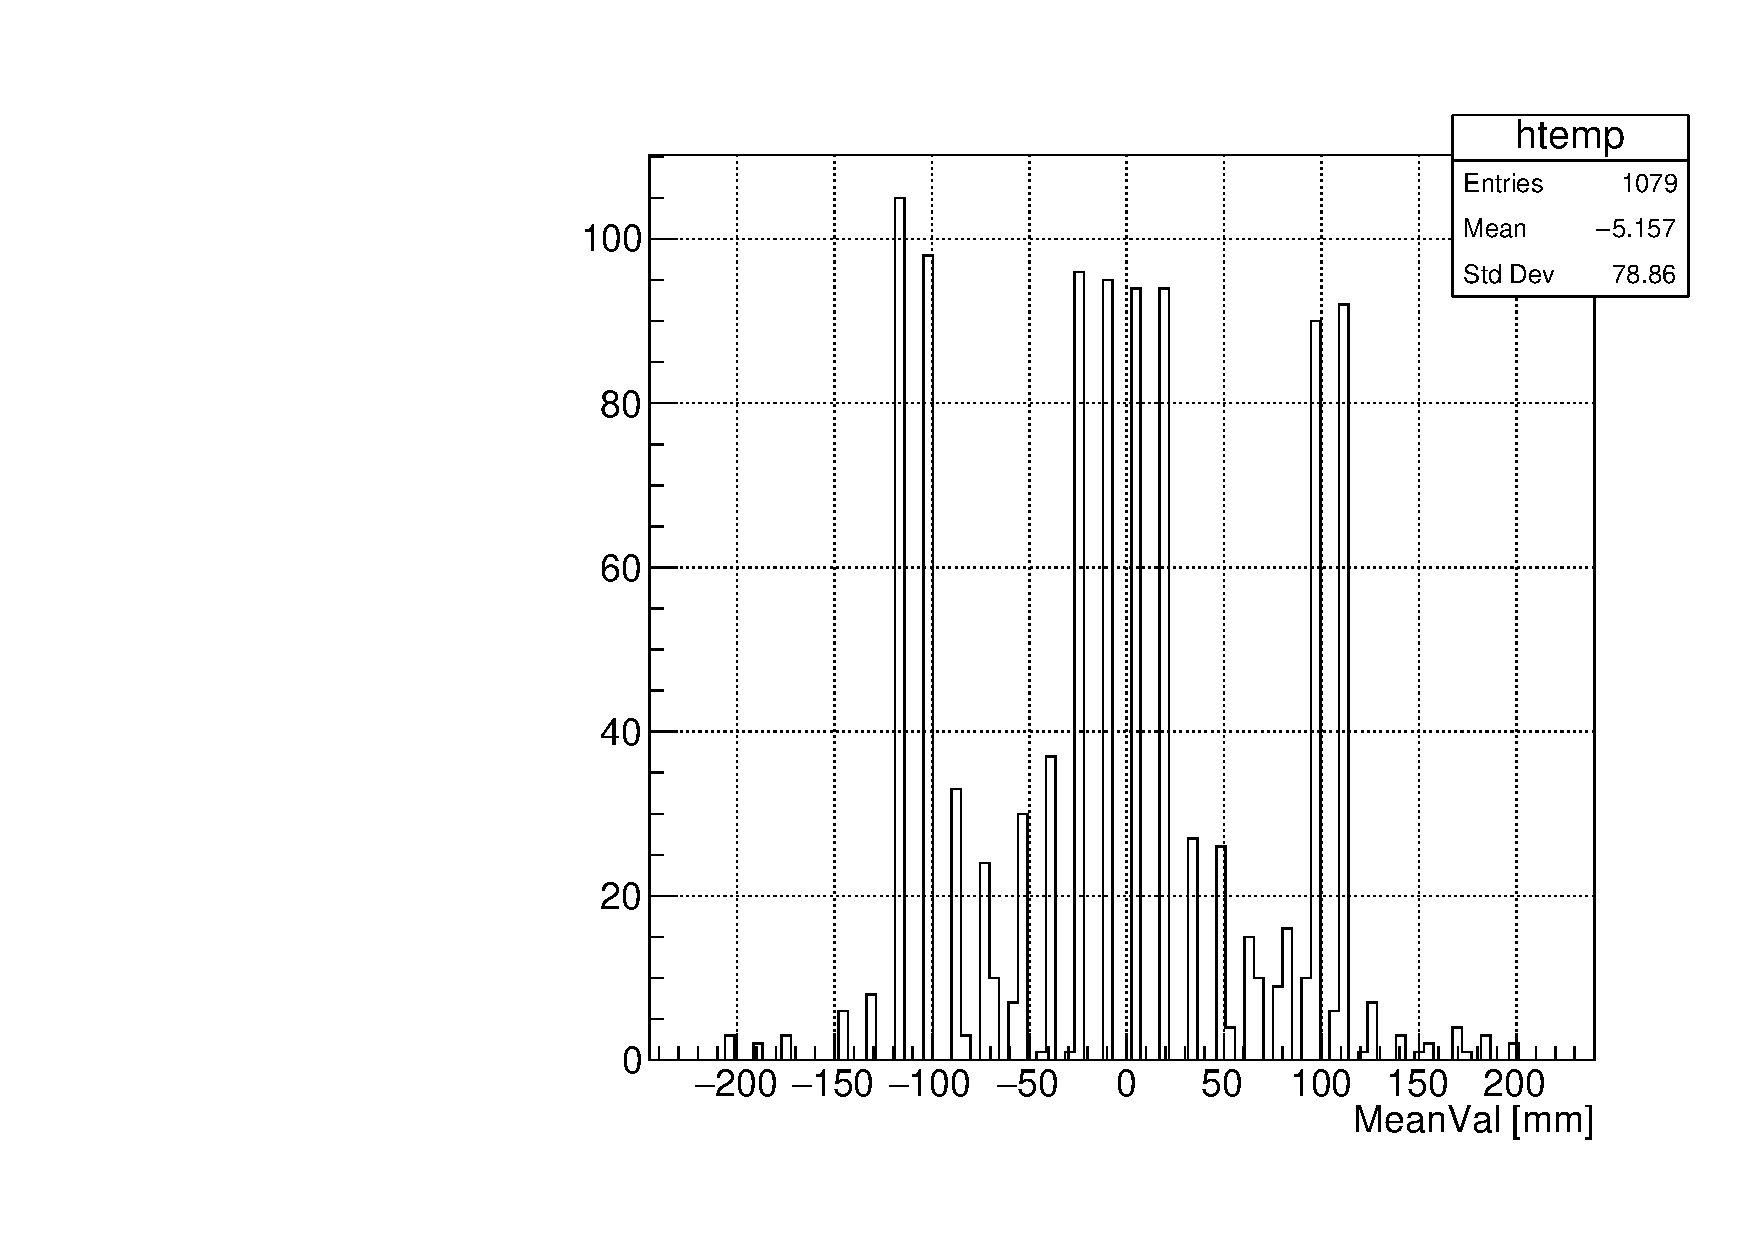
\includegraphics[width=.4\linewidth]{plots/2018/ZMeanVal.pdf}
    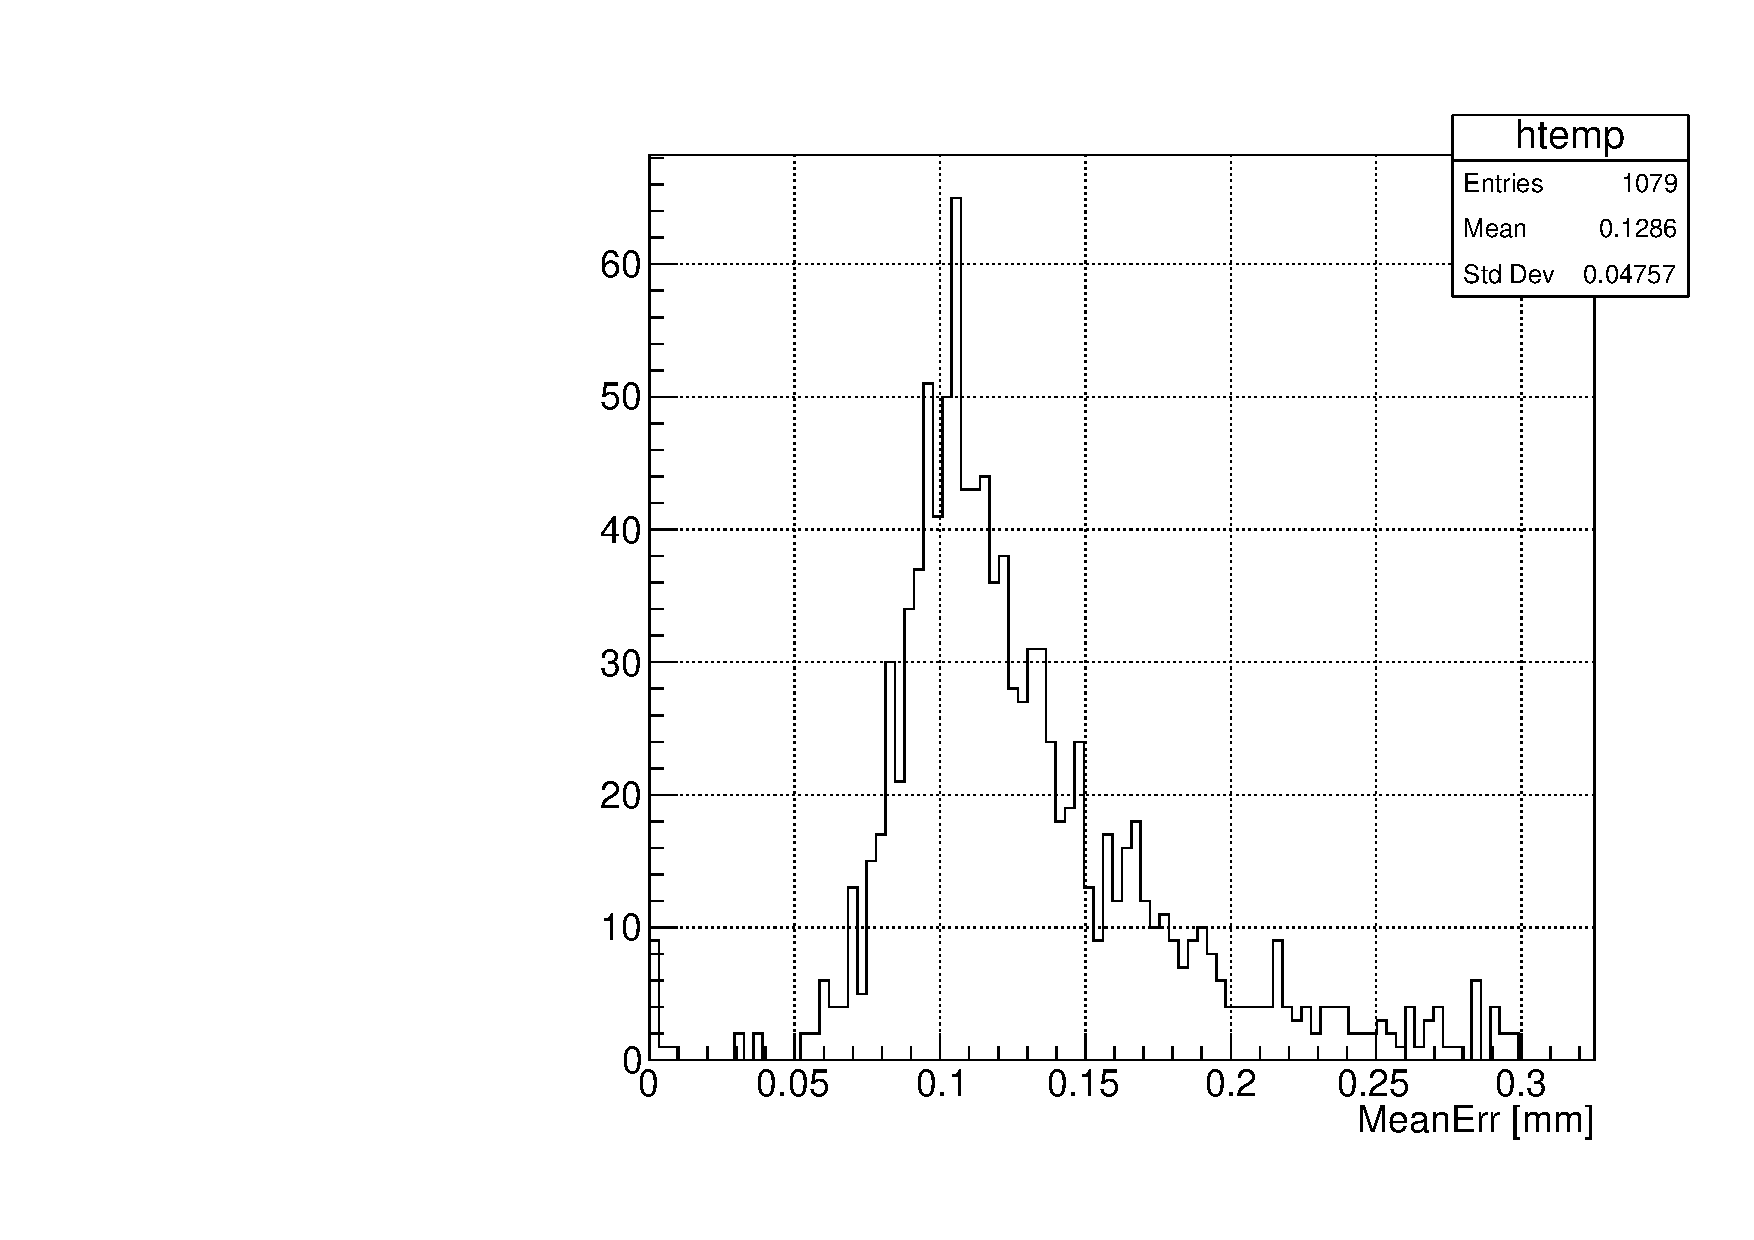
\includegraphics[width=.4\linewidth]{plots/2018/ZMeanErr.pdf}\\
    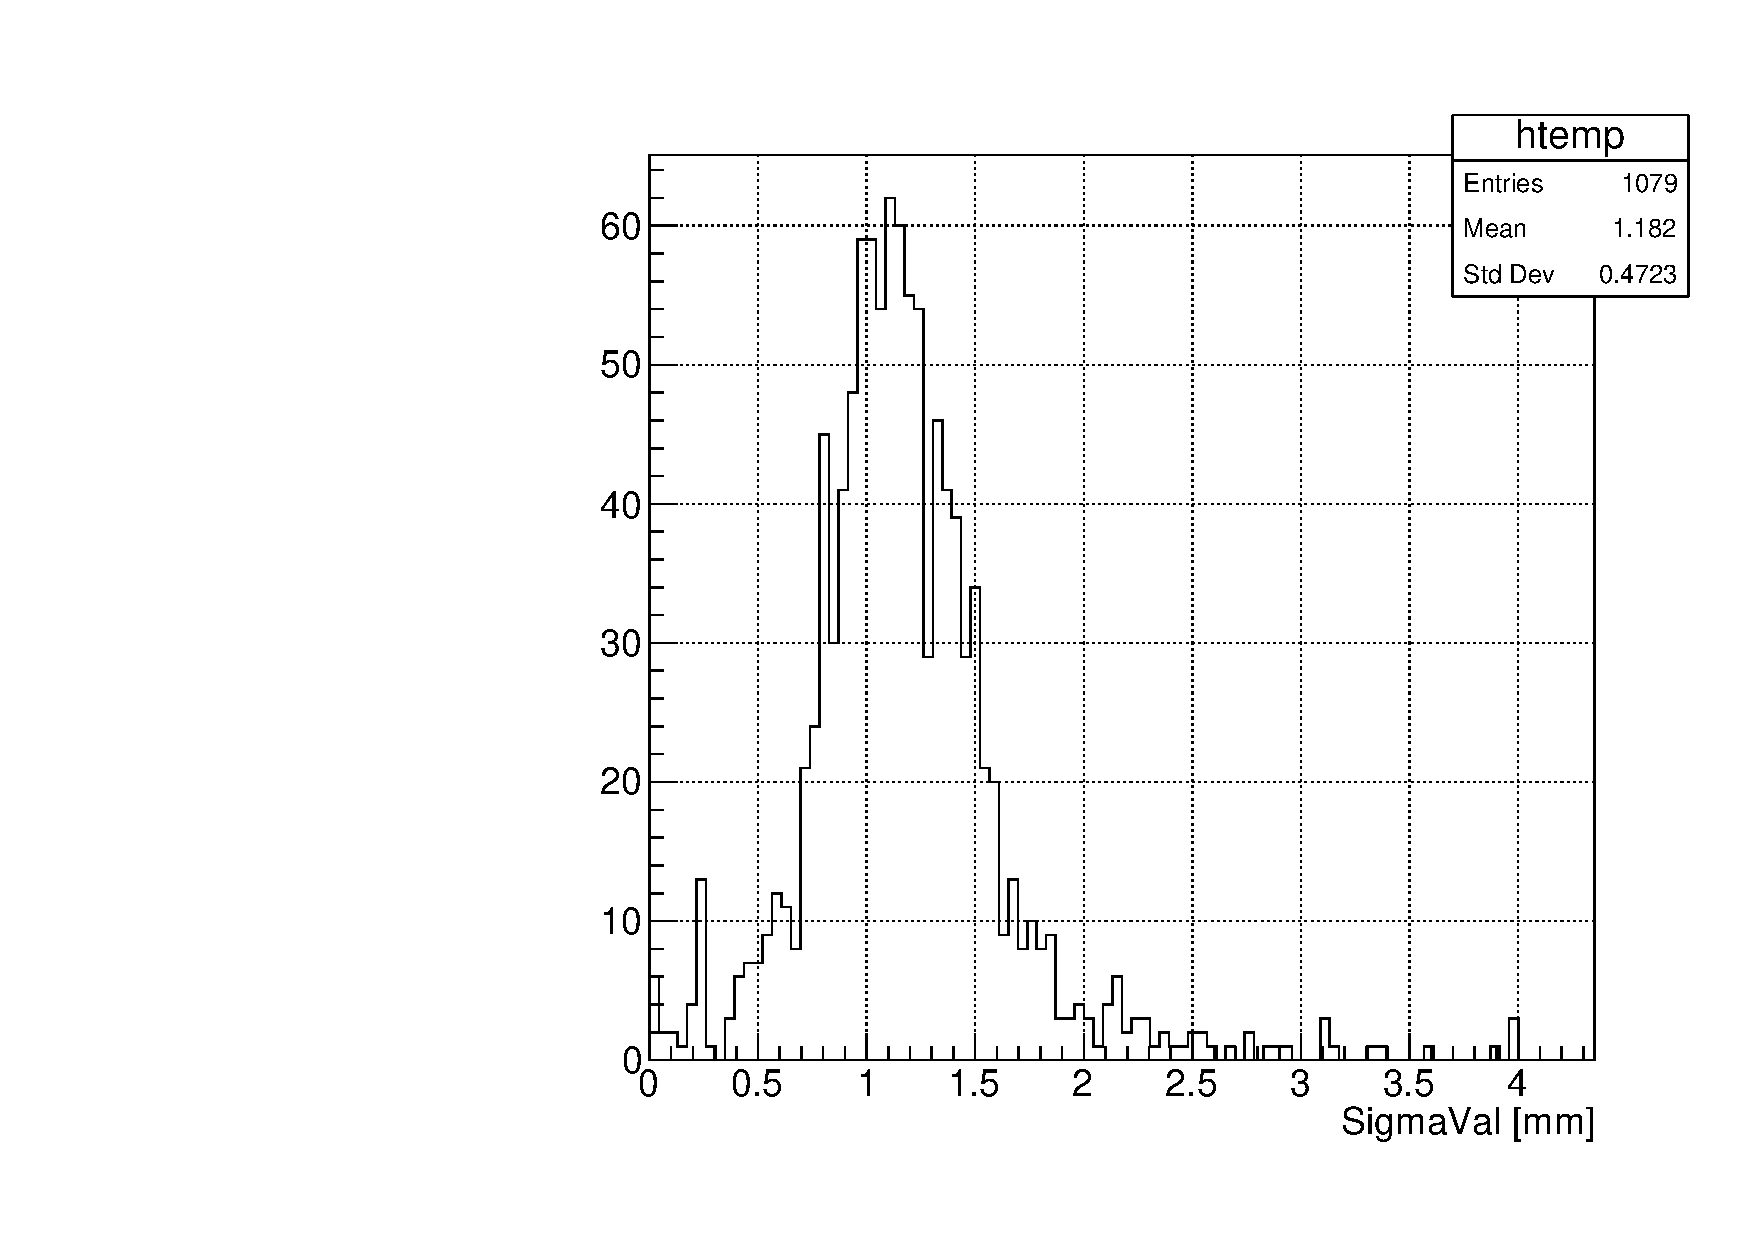
\includegraphics[width=.4\linewidth]{plots/2018/ZSigmaVal.pdf}
    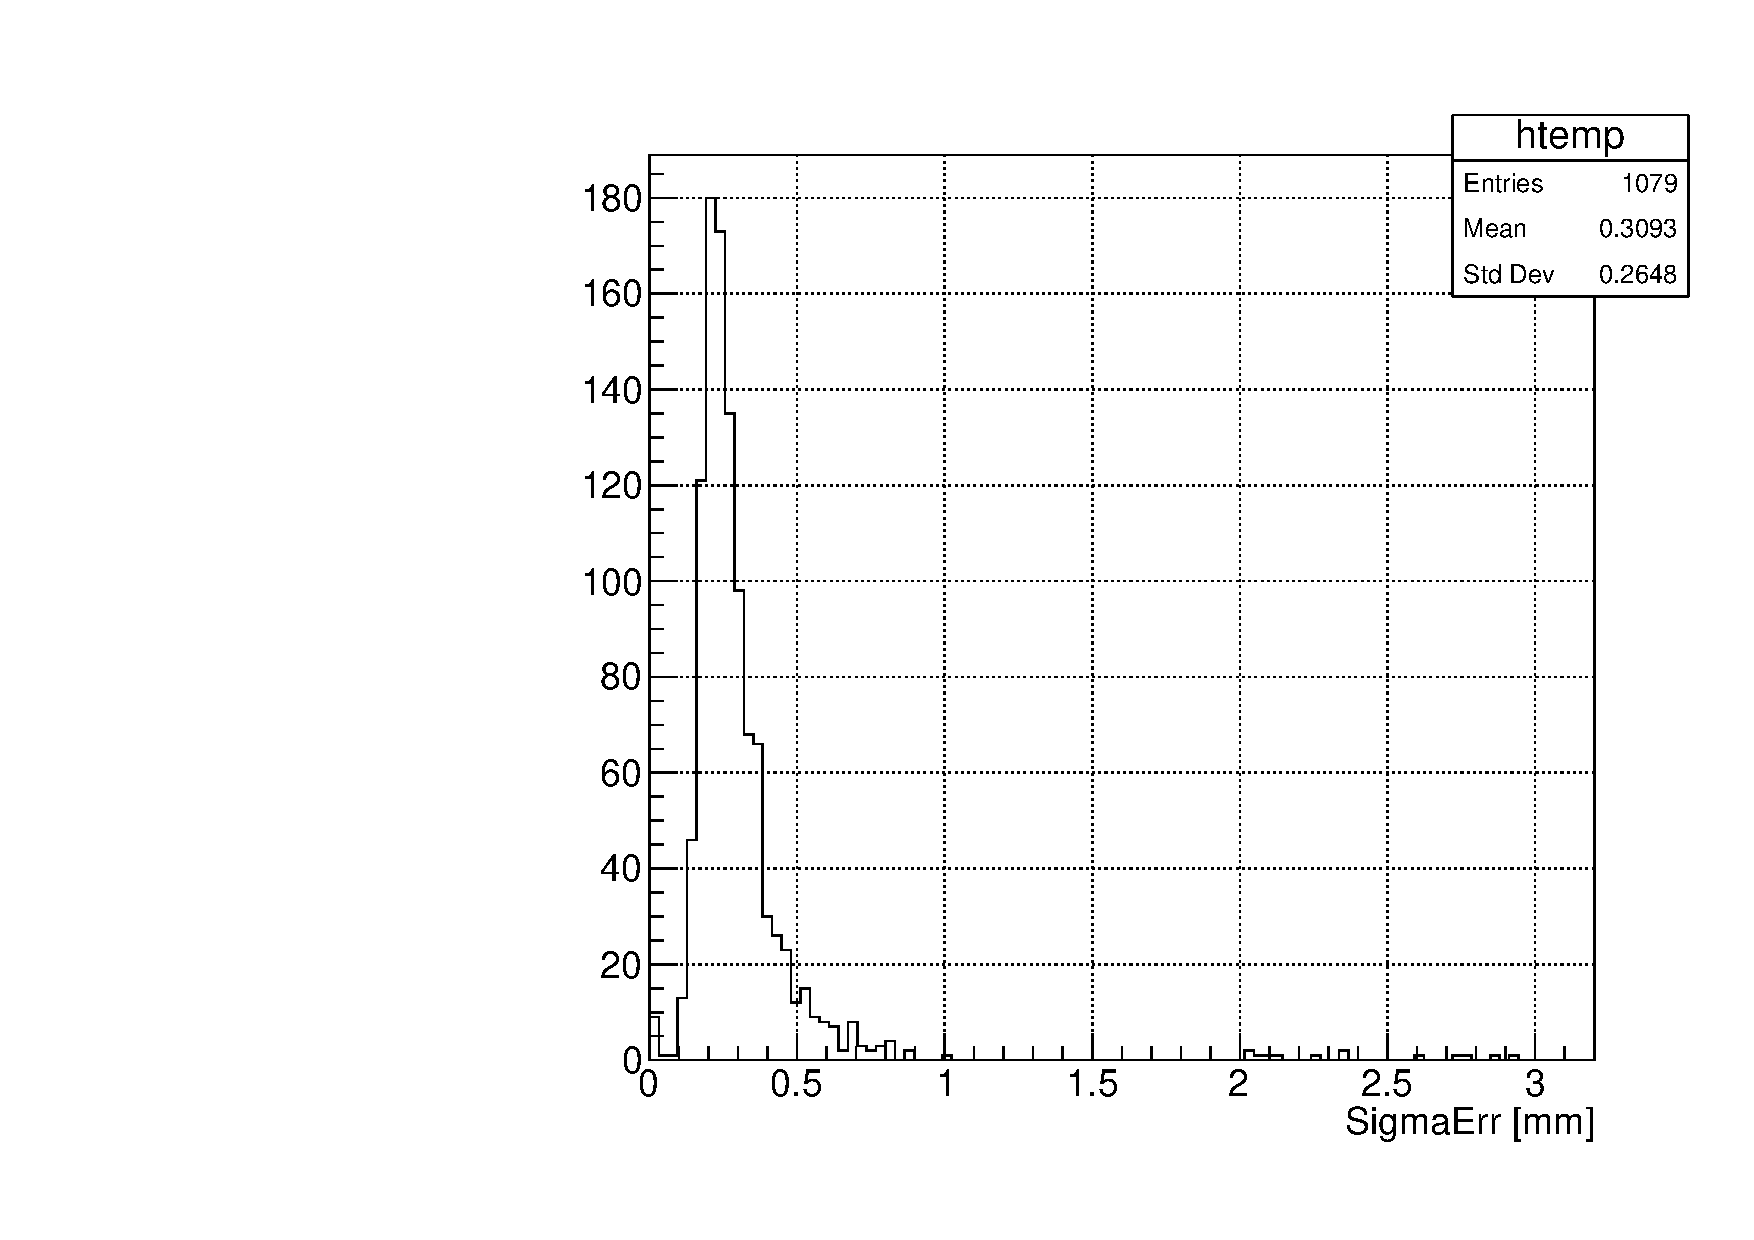
\includegraphics[width=.4\linewidth]{plots/2018/ZSigmaErr.pdf}\\
    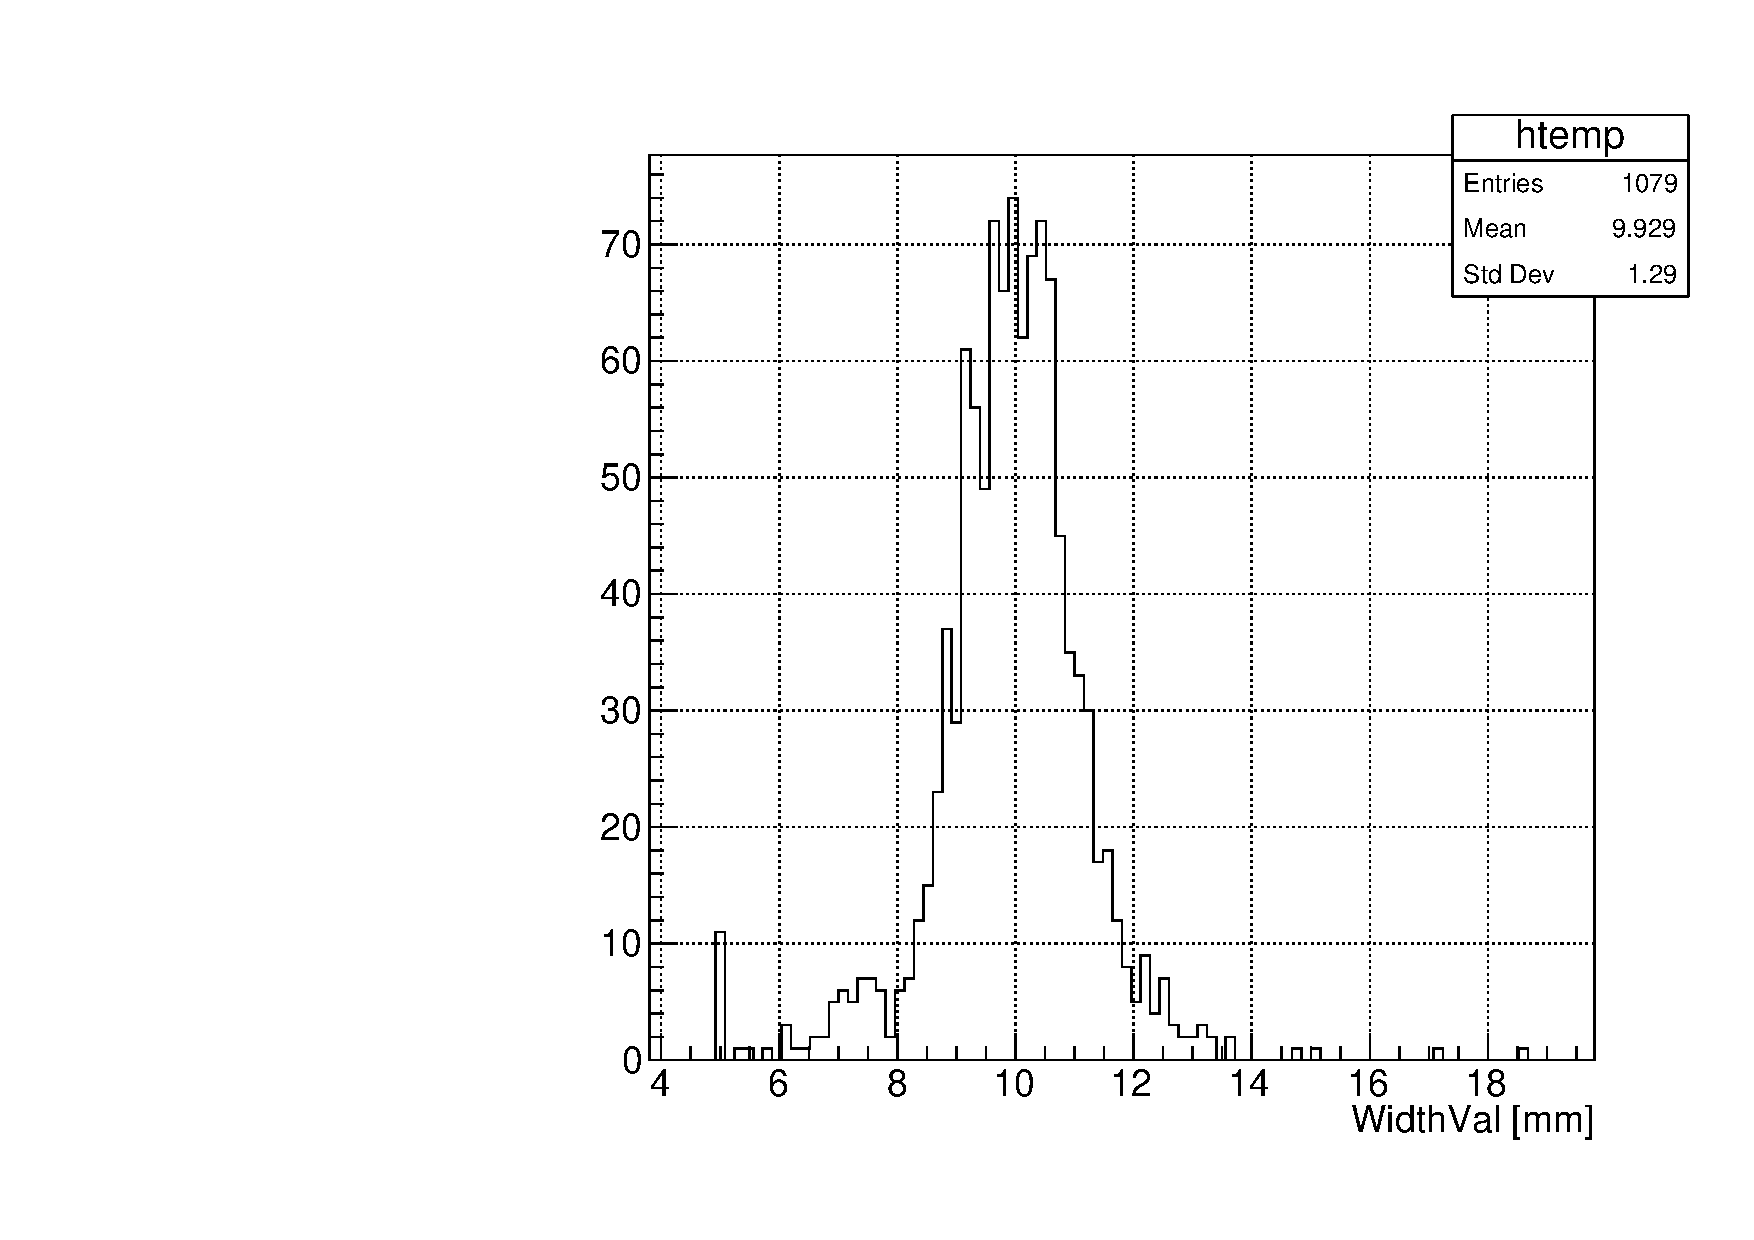
\includegraphics[width=.4\linewidth]{plots/2018/ZWidthVal.pdf}
    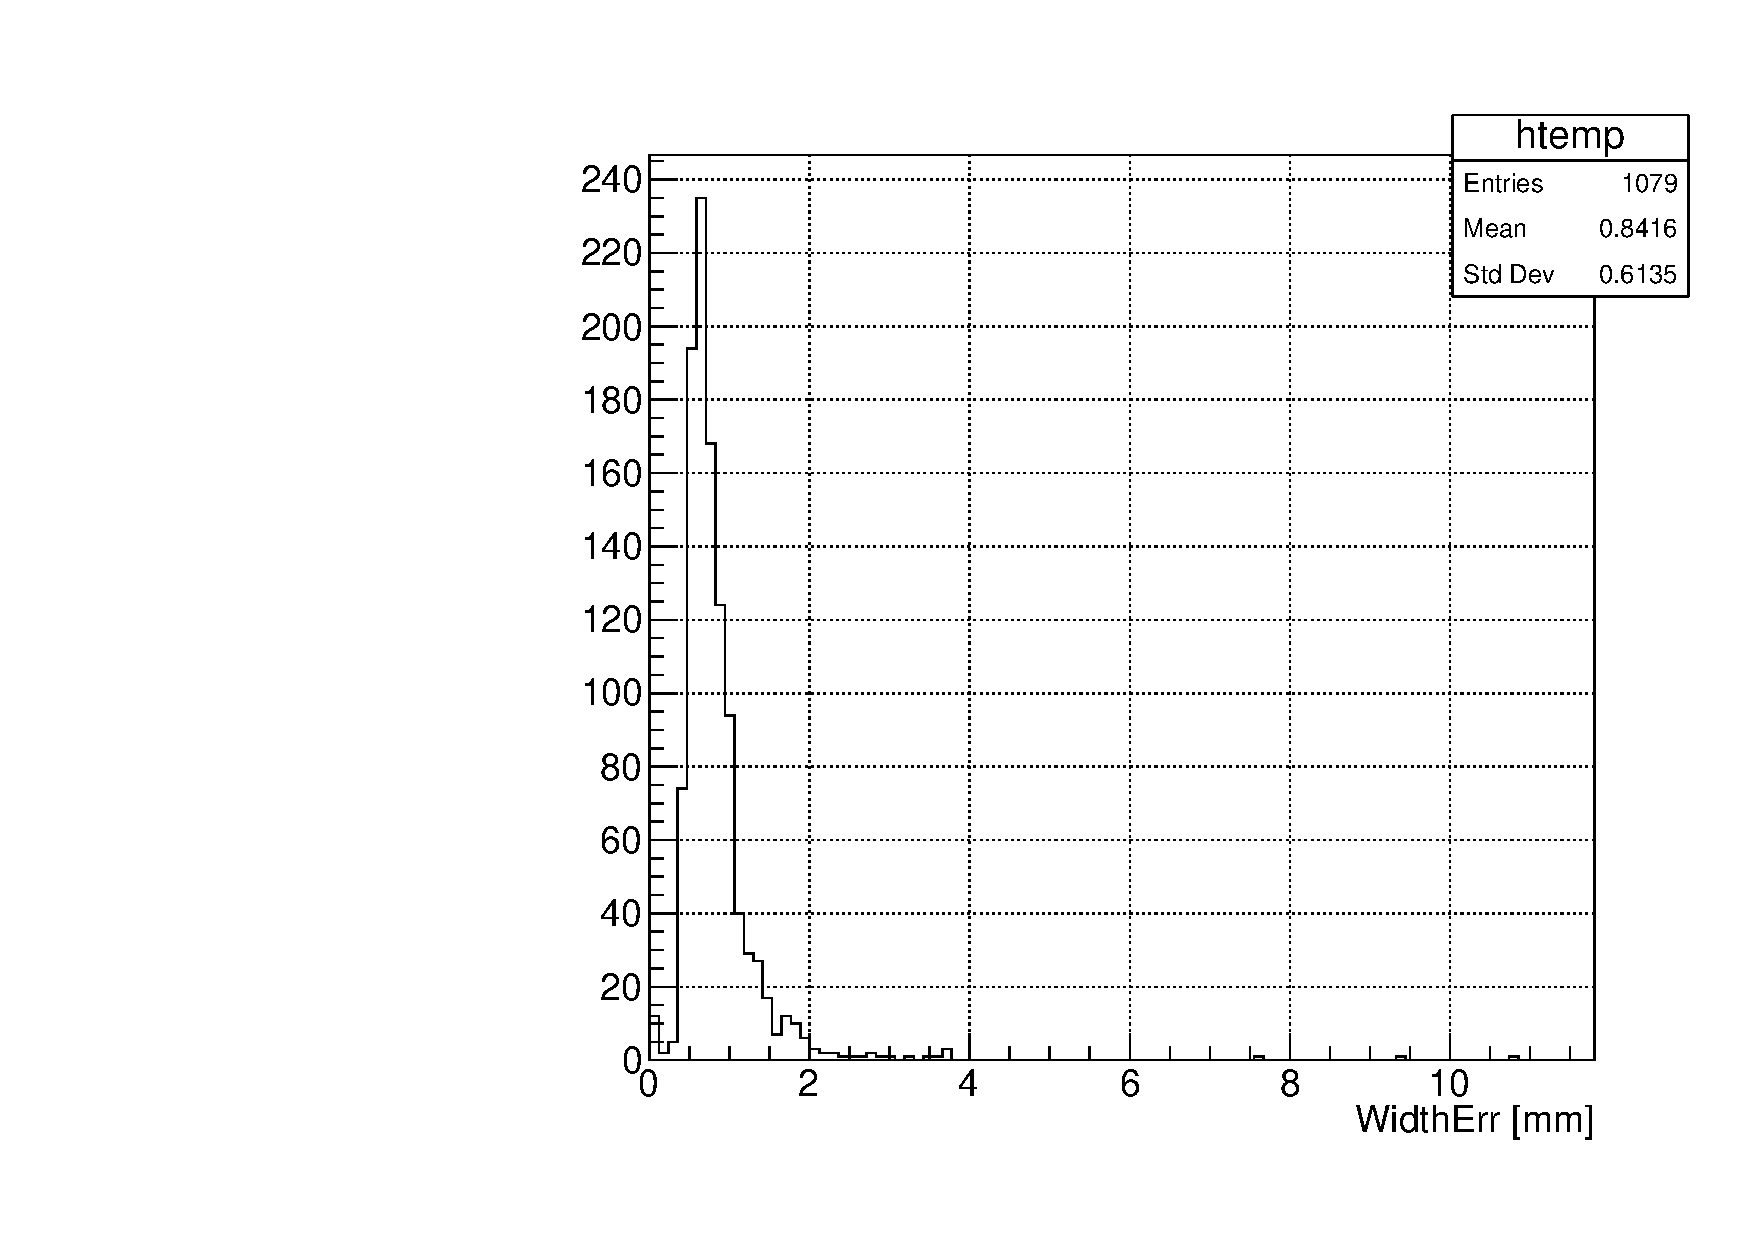
\includegraphics[width=.4\linewidth]{plots/2018/ZWidthErr.pdf}\\
    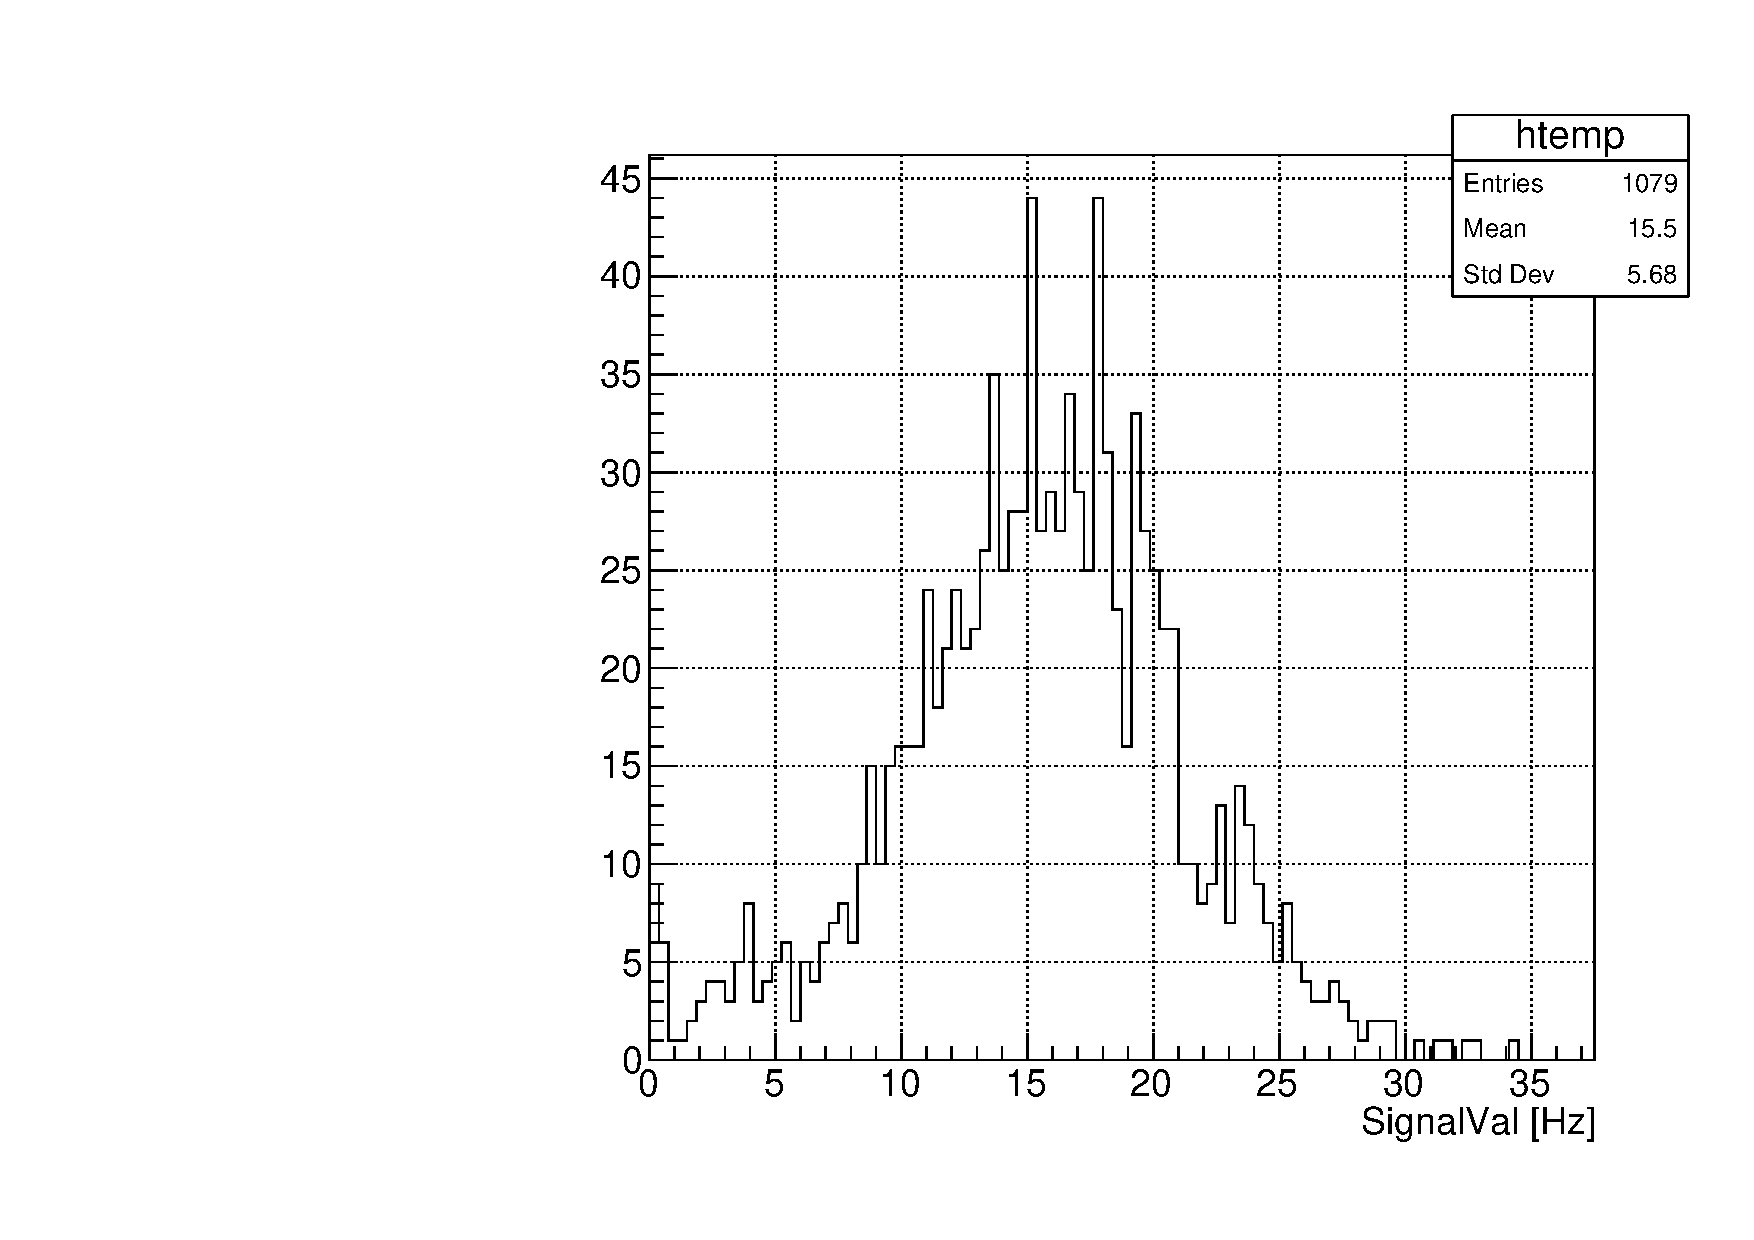
\includegraphics[width=.4\linewidth]{plots/2018/ZSignalVal.pdf}
    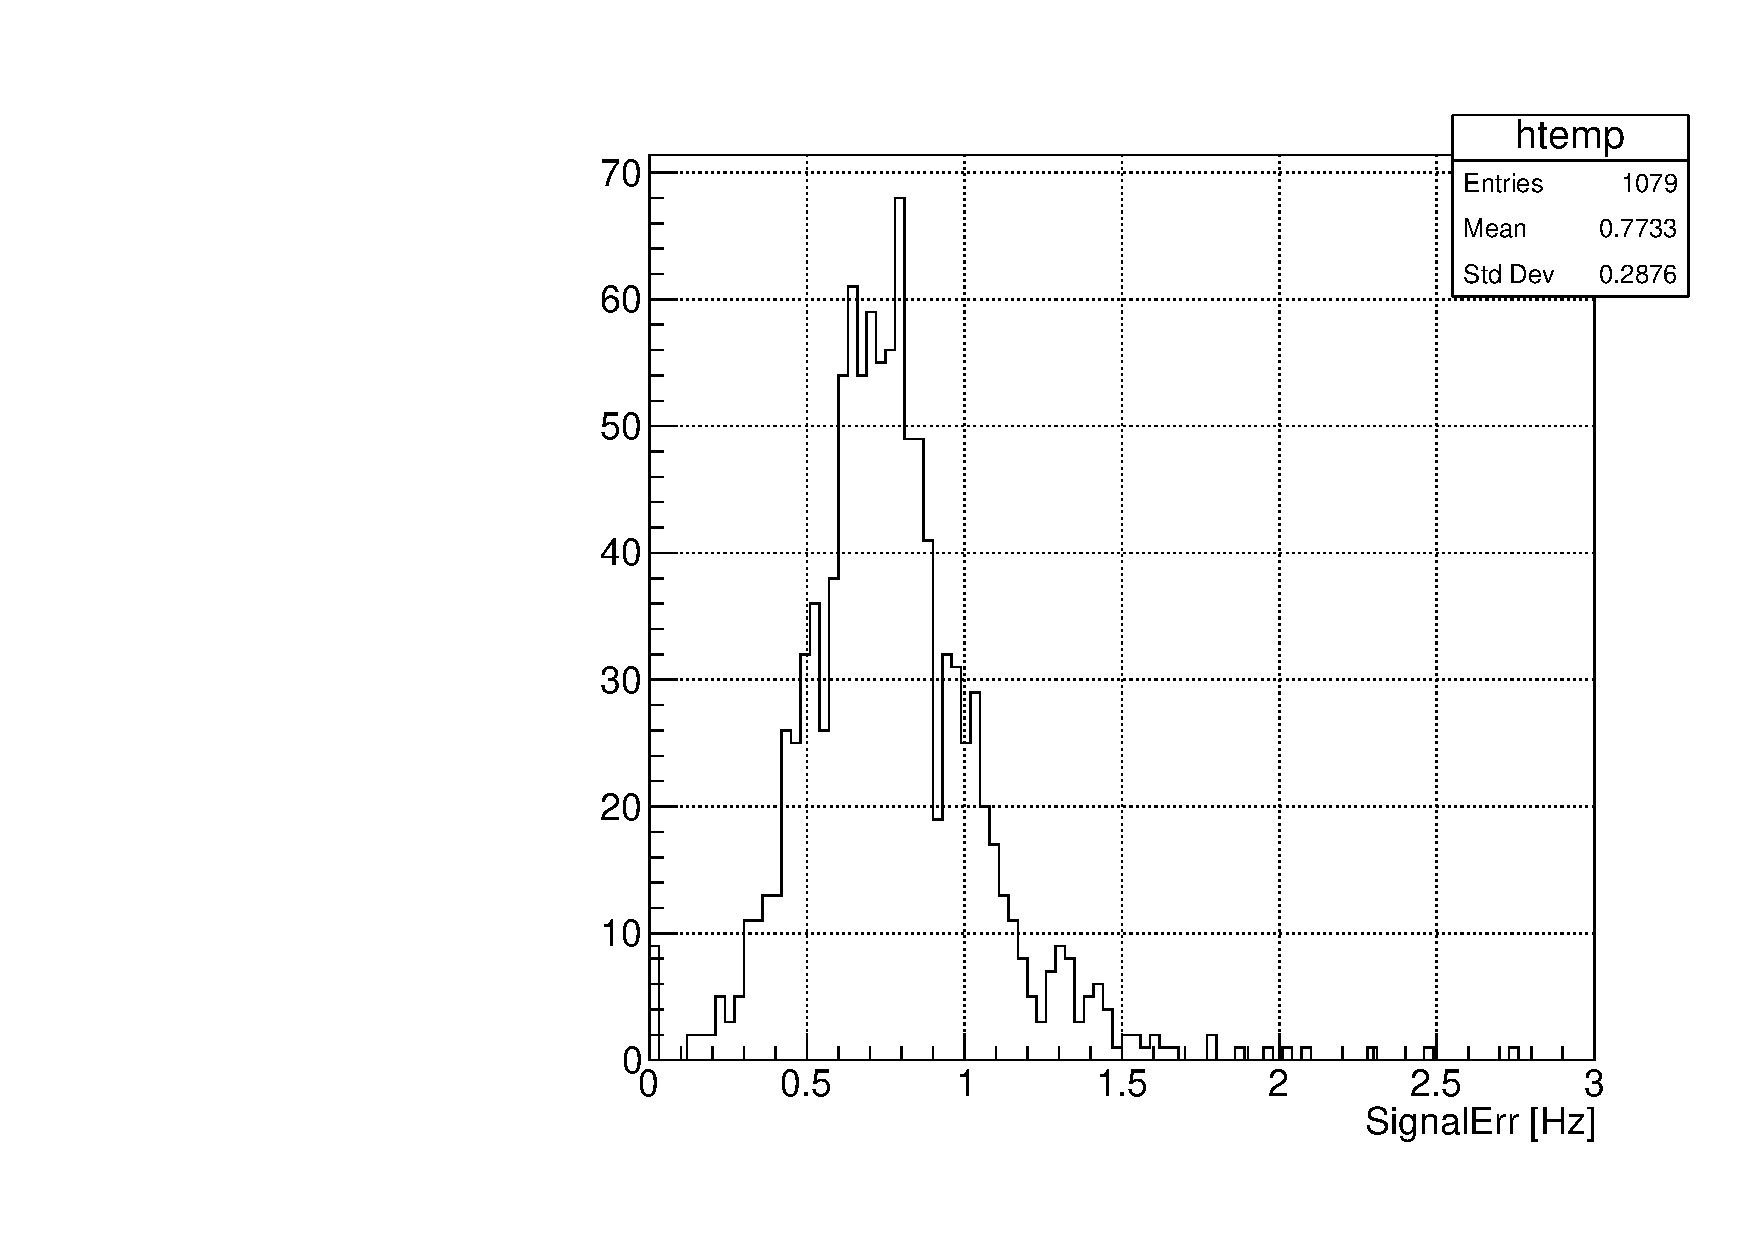
\includegraphics[width=.4\linewidth]{plots/2018/ZSignalErr.pdf}\\
    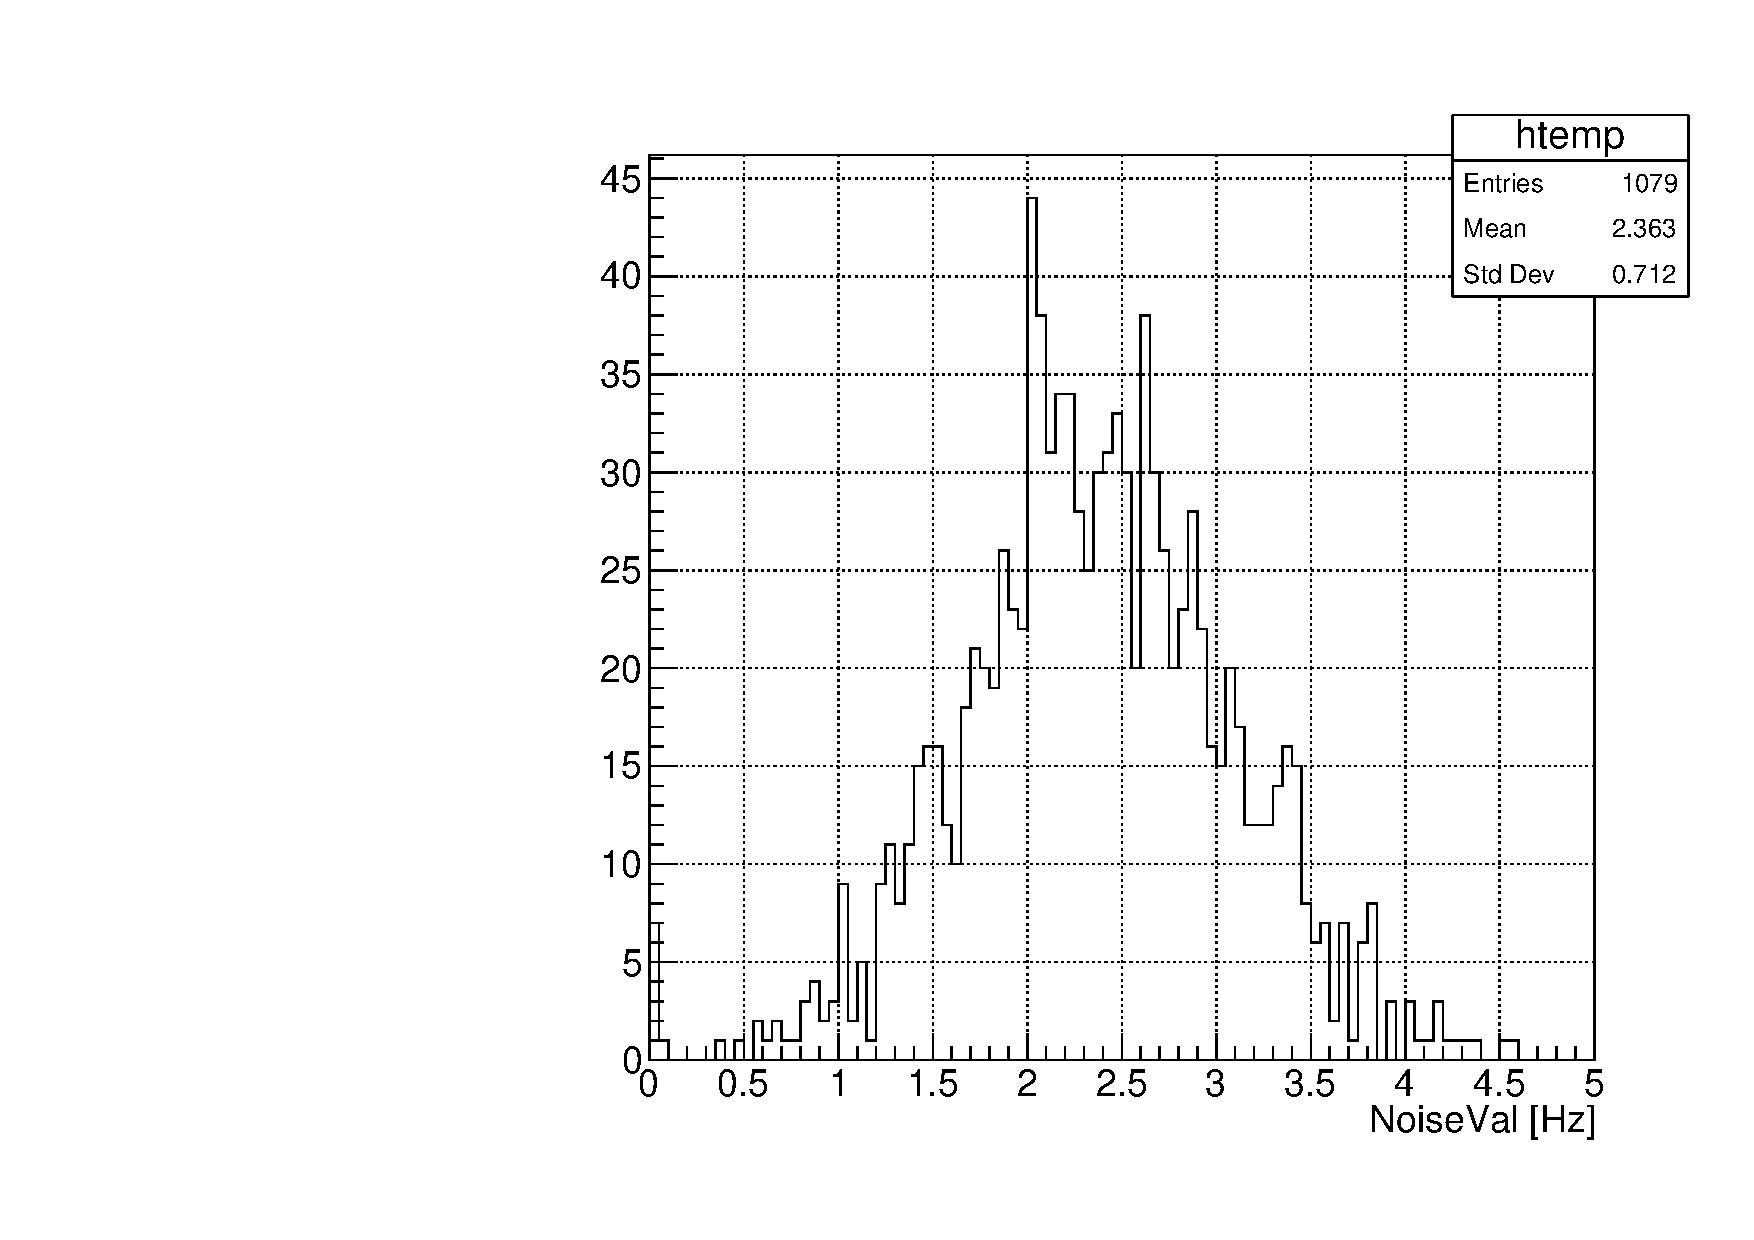
\includegraphics[width=.4\linewidth]{plots/2018/ZNoiseVal.pdf}
    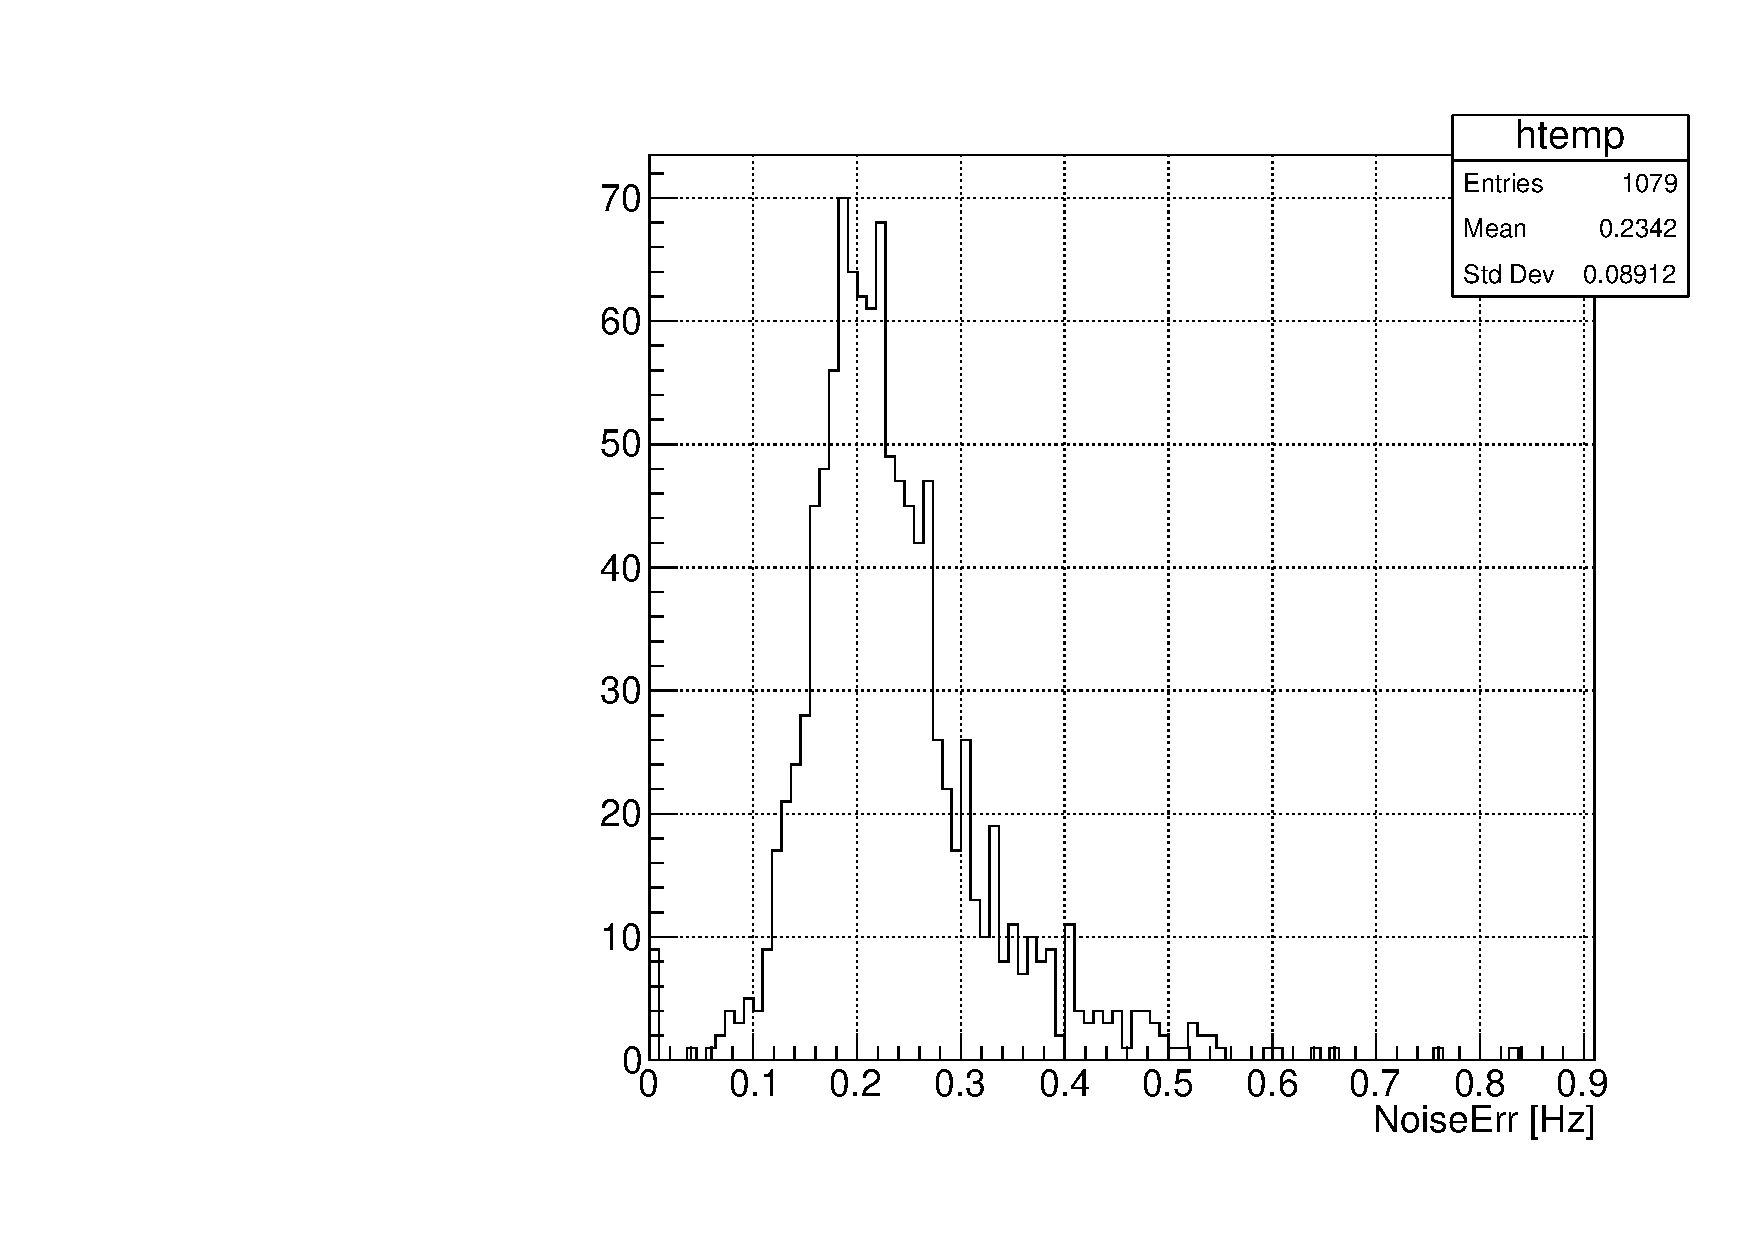
\includegraphics[width=.4\linewidth]{plots/2018/ZNoiseErr.pdf}
    \caption{Fitted parameter values (left) and errors (right) for Z position fits.}
    \label{fig:zfitpars}
\end{figure}

\begin{figure}[h]
    \centering
    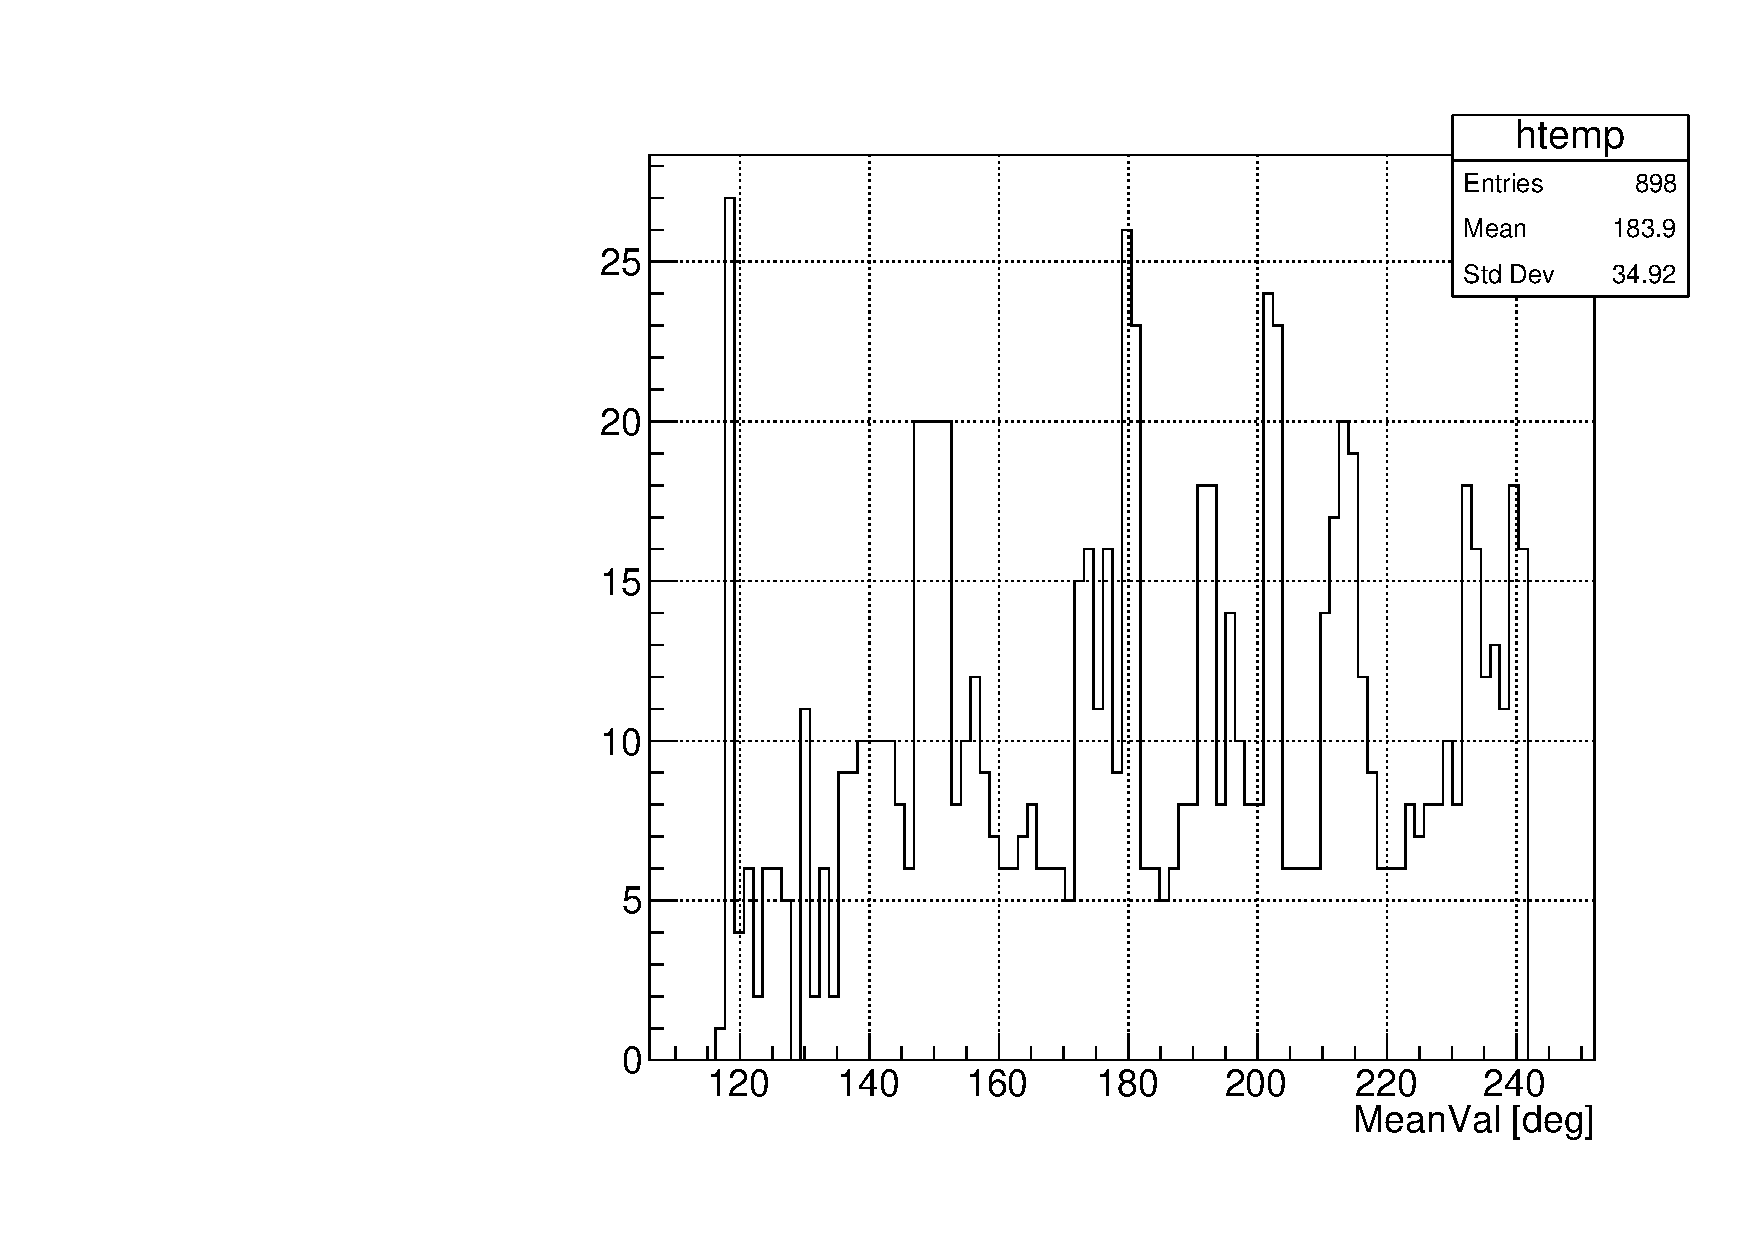
\includegraphics[width=.4\linewidth]{plots/2018/PhiMeanVal.pdf}
    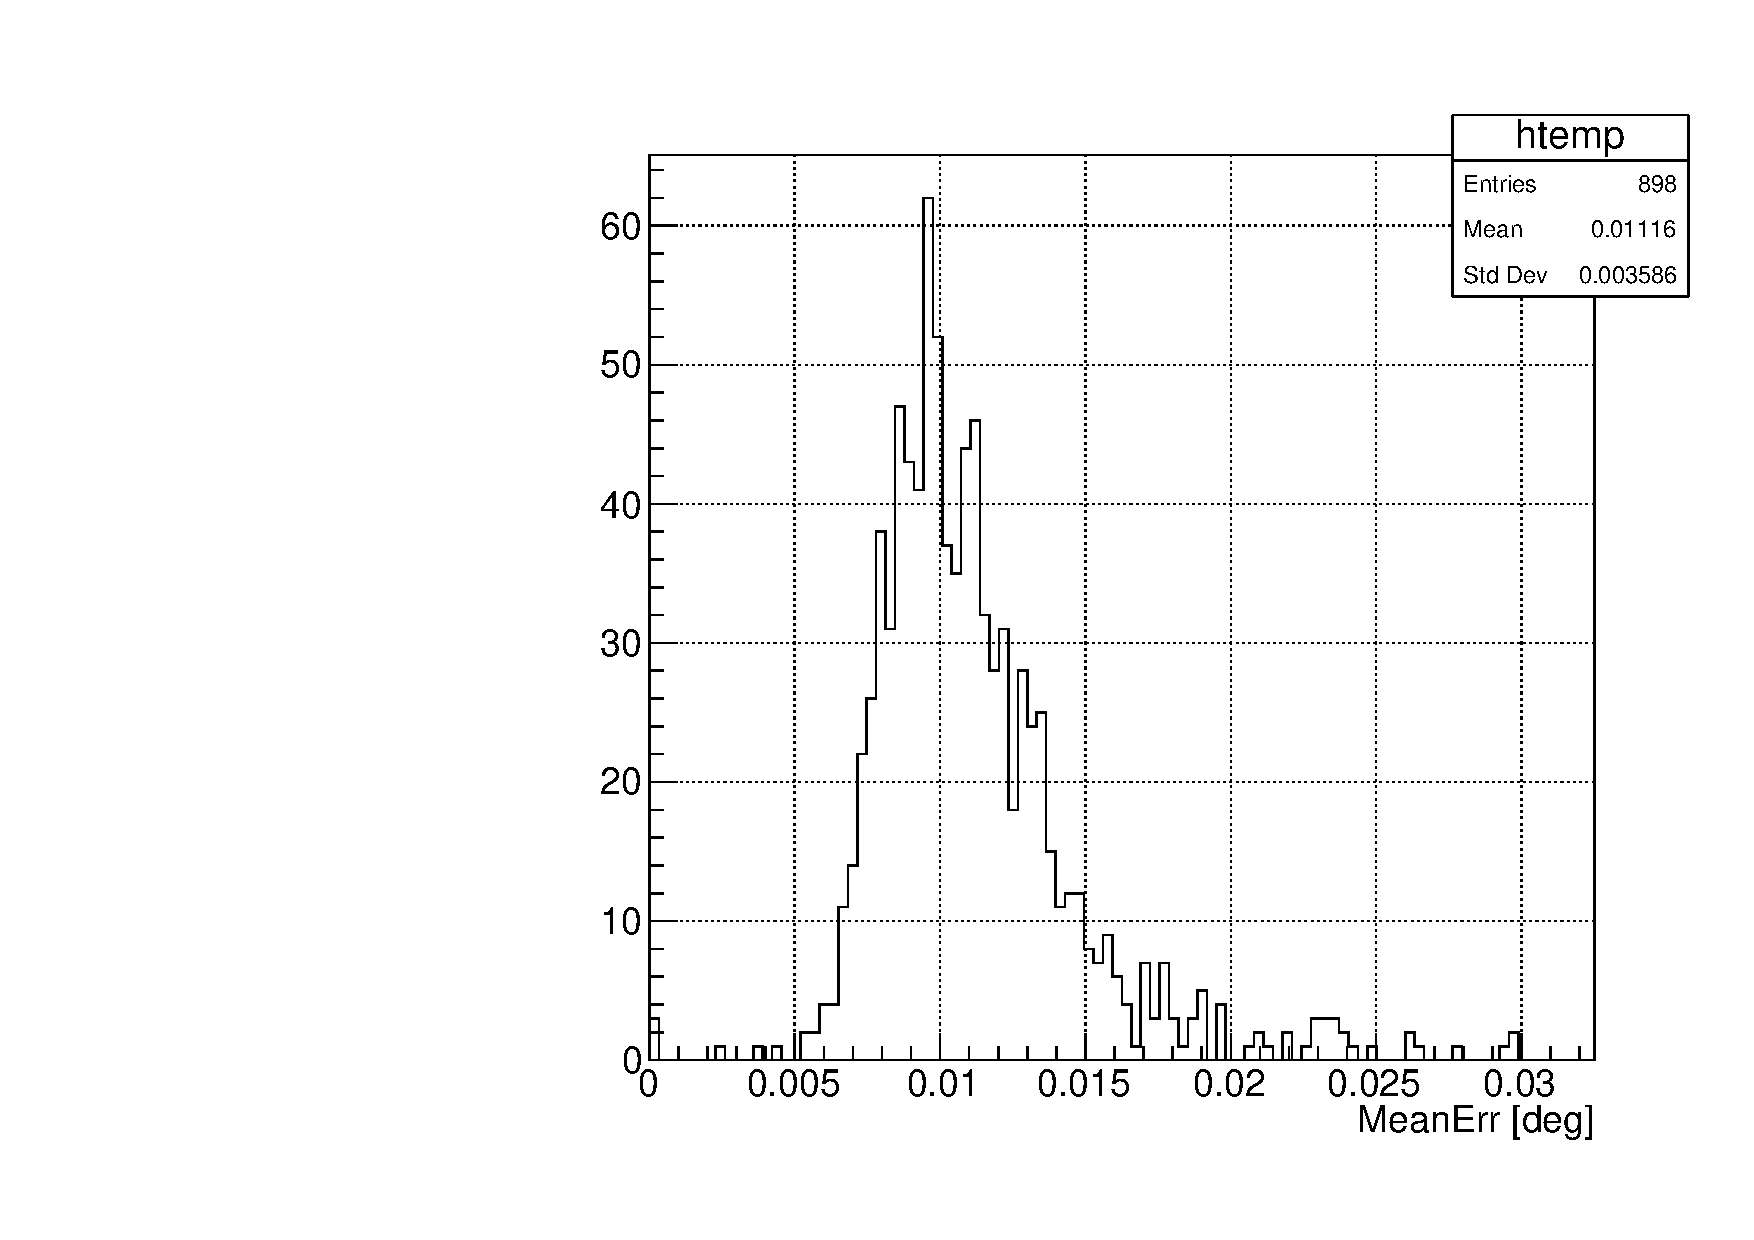
\includegraphics[width=.4\linewidth]{plots/2018/PhiMeanErr.pdf}\\
    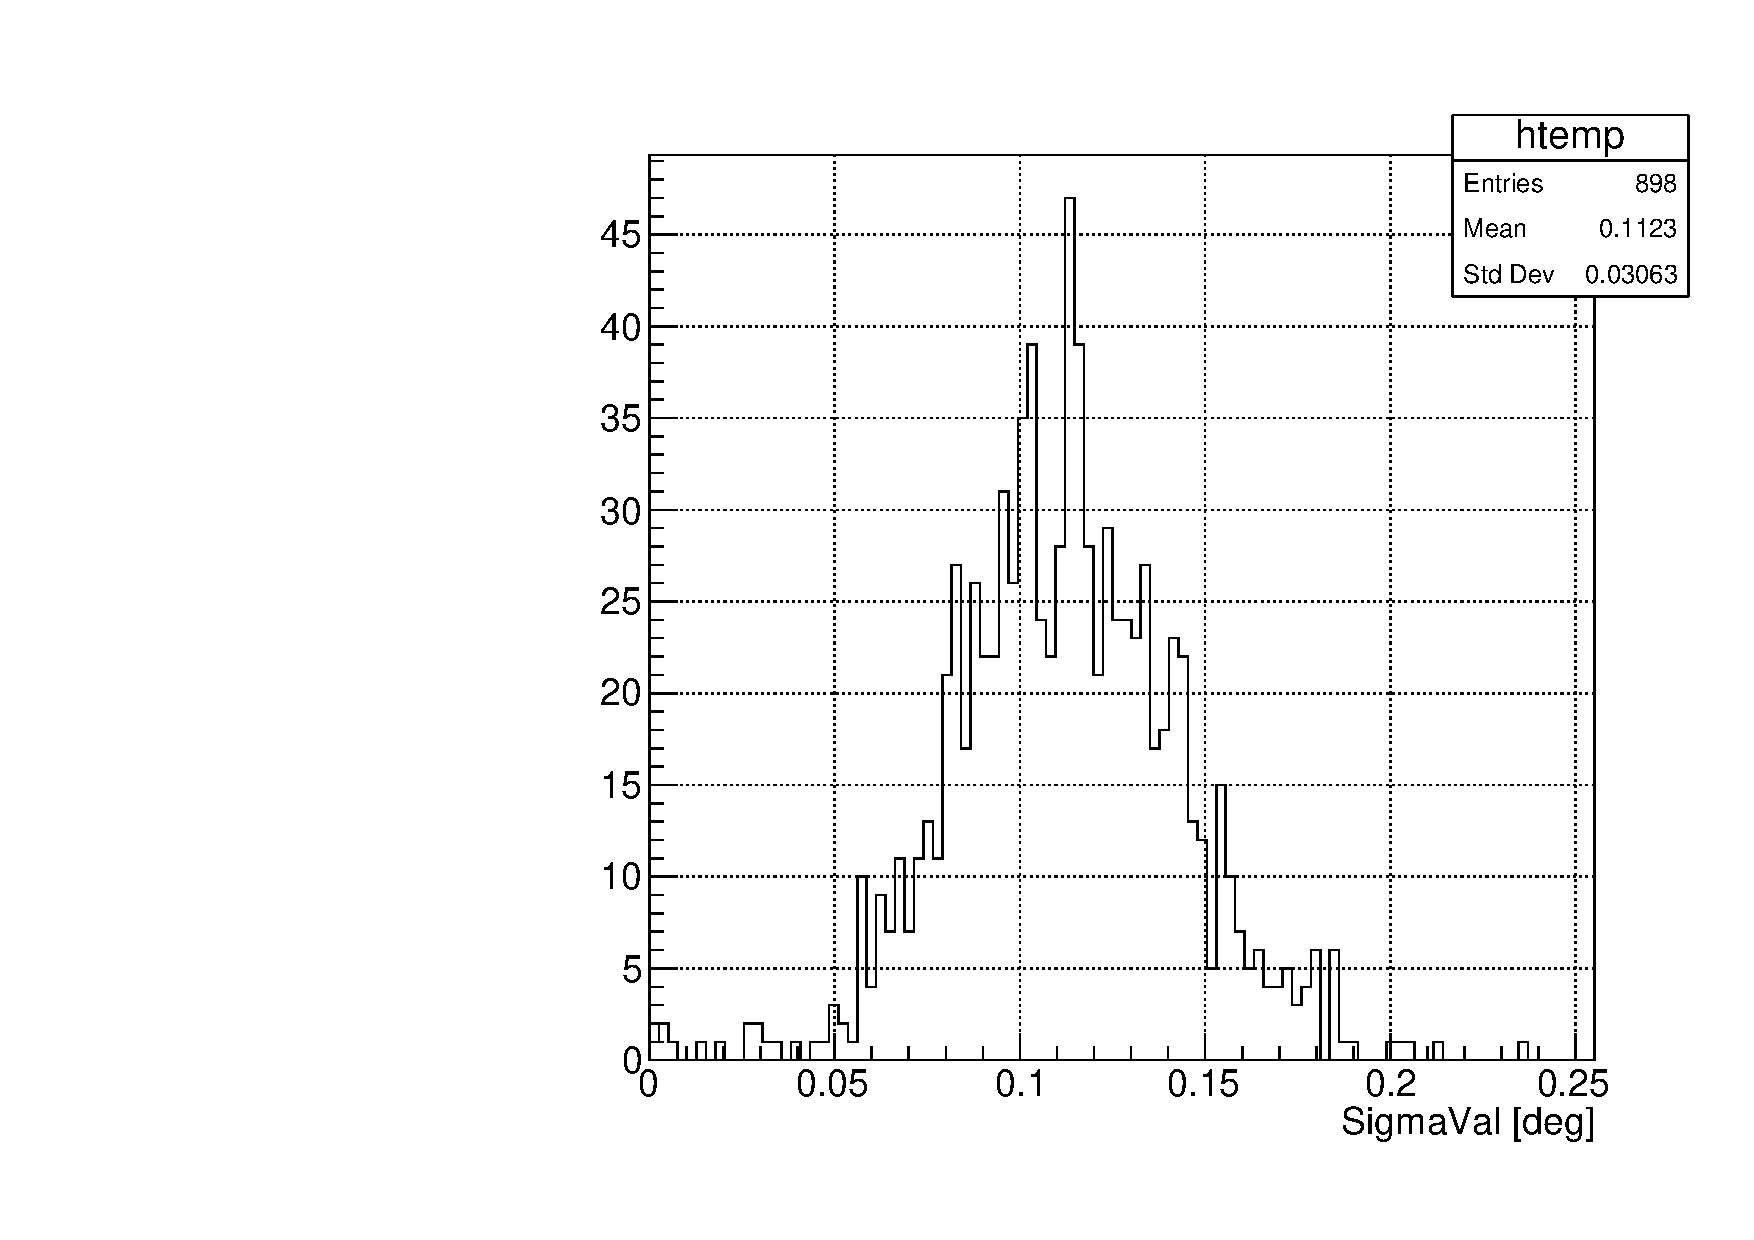
\includegraphics[width=.4\linewidth]{plots/2018/PhiSigmaVal.pdf}
    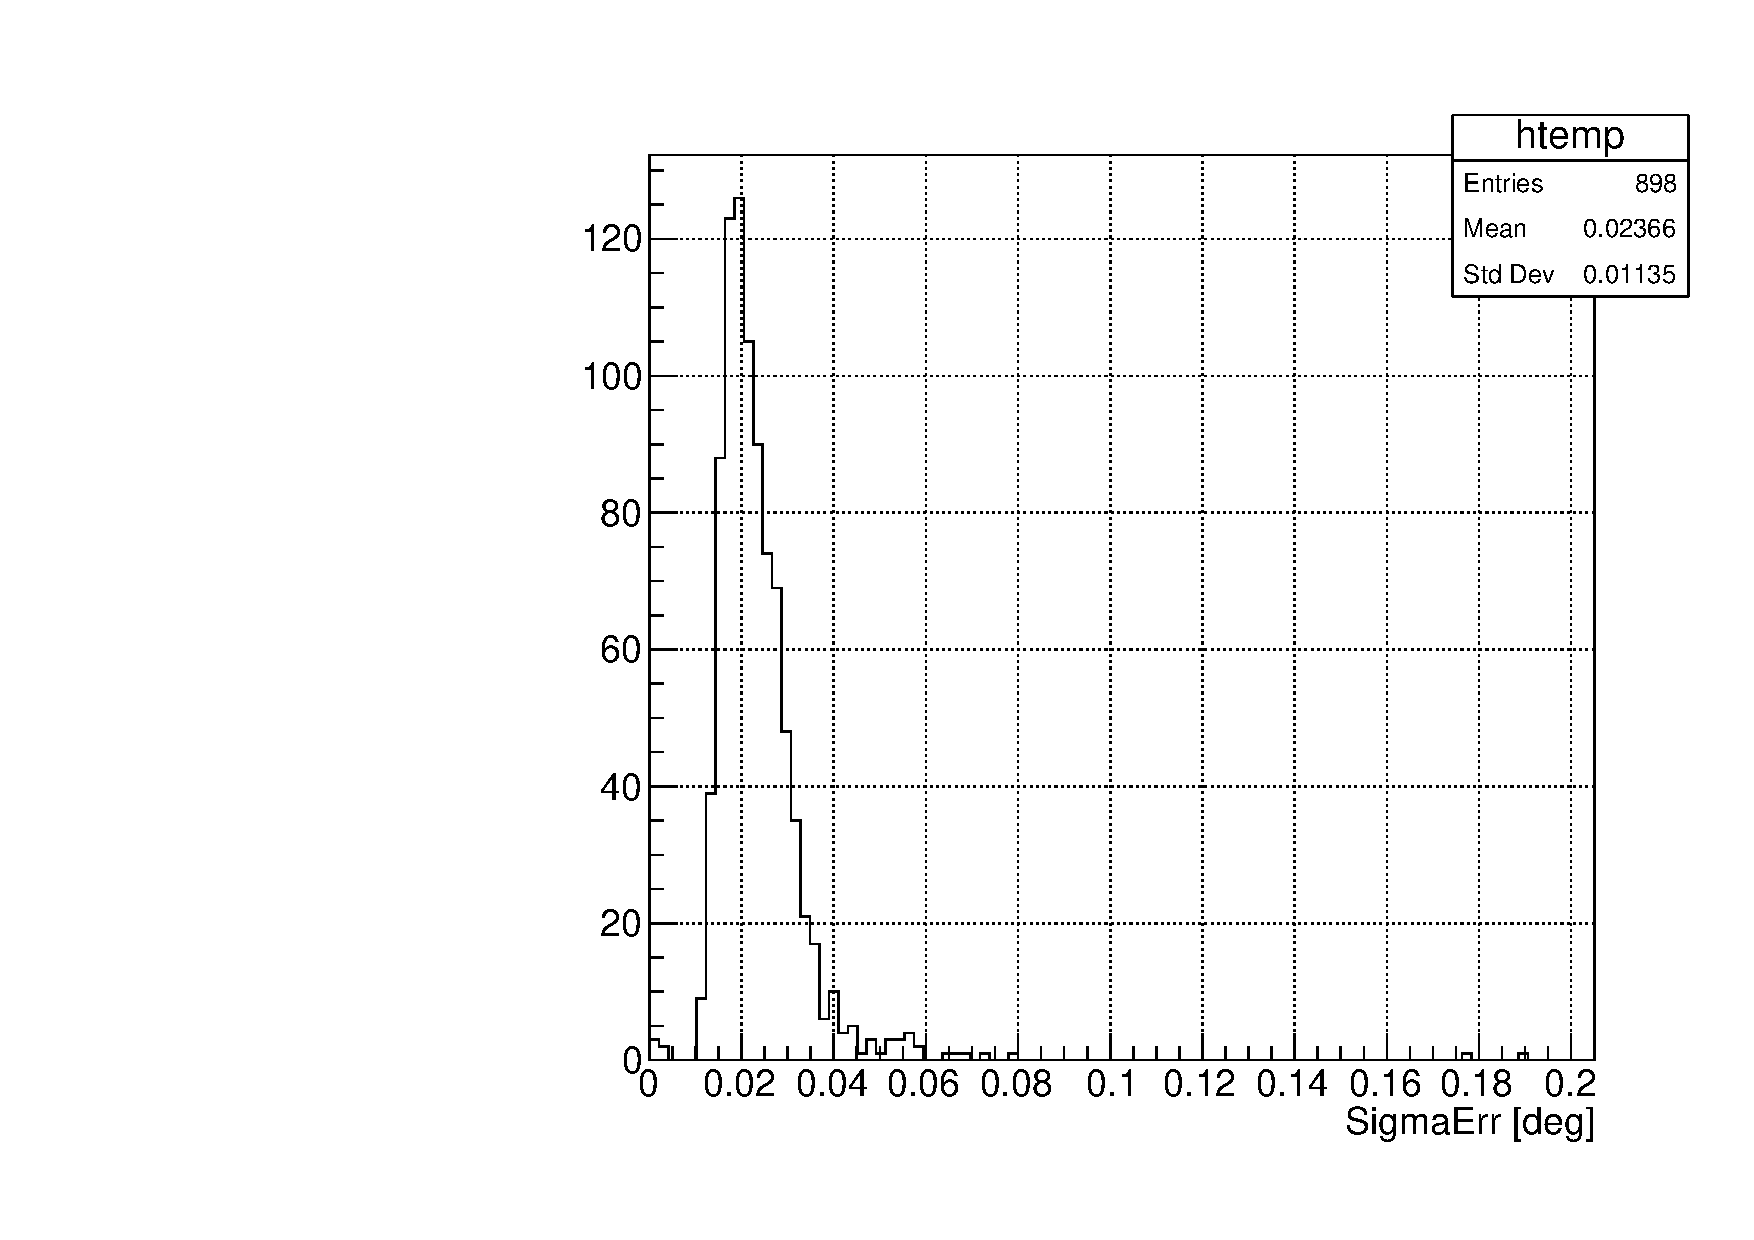
\includegraphics[width=.4\linewidth]{plots/2018/PhiSigmaErr.pdf}\\
    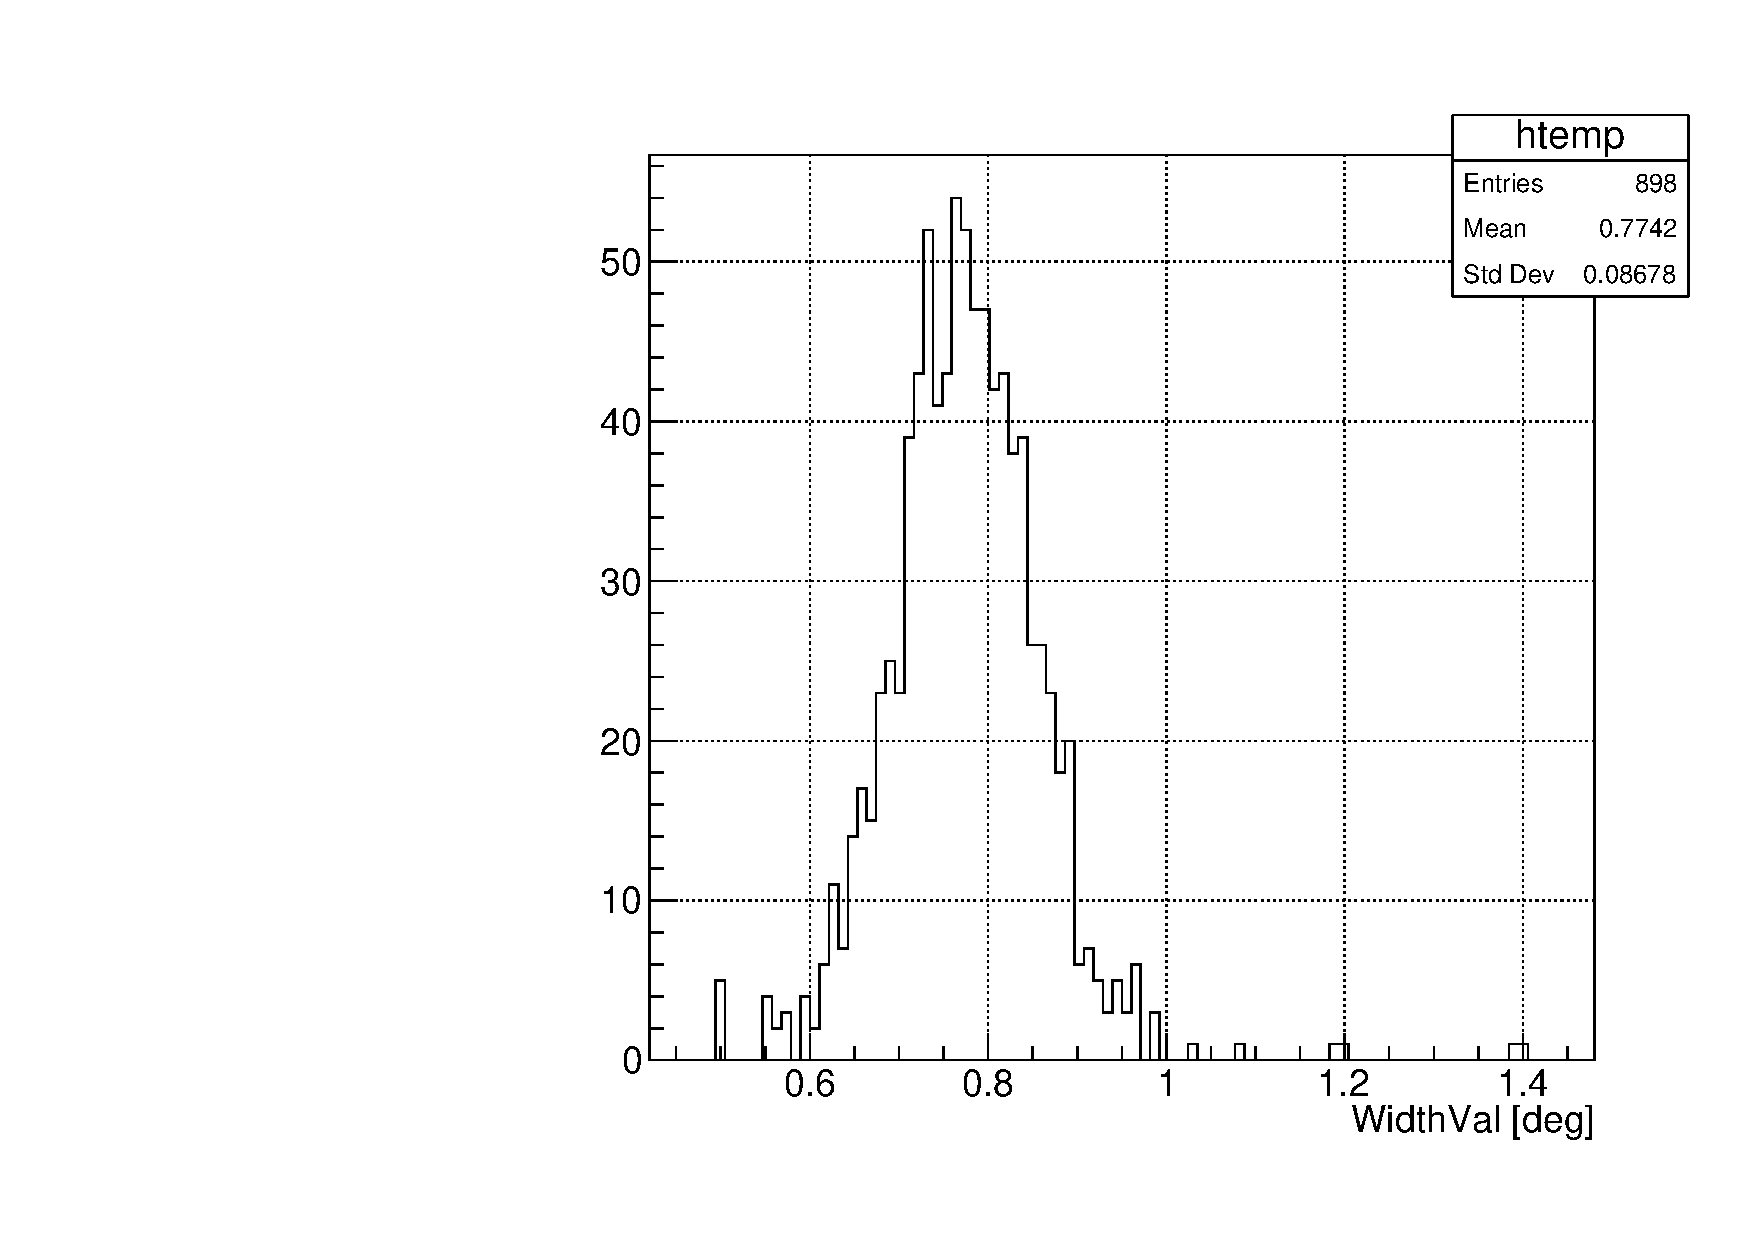
\includegraphics[width=.4\linewidth]{plots/2018/PhiWidthVal.pdf}
    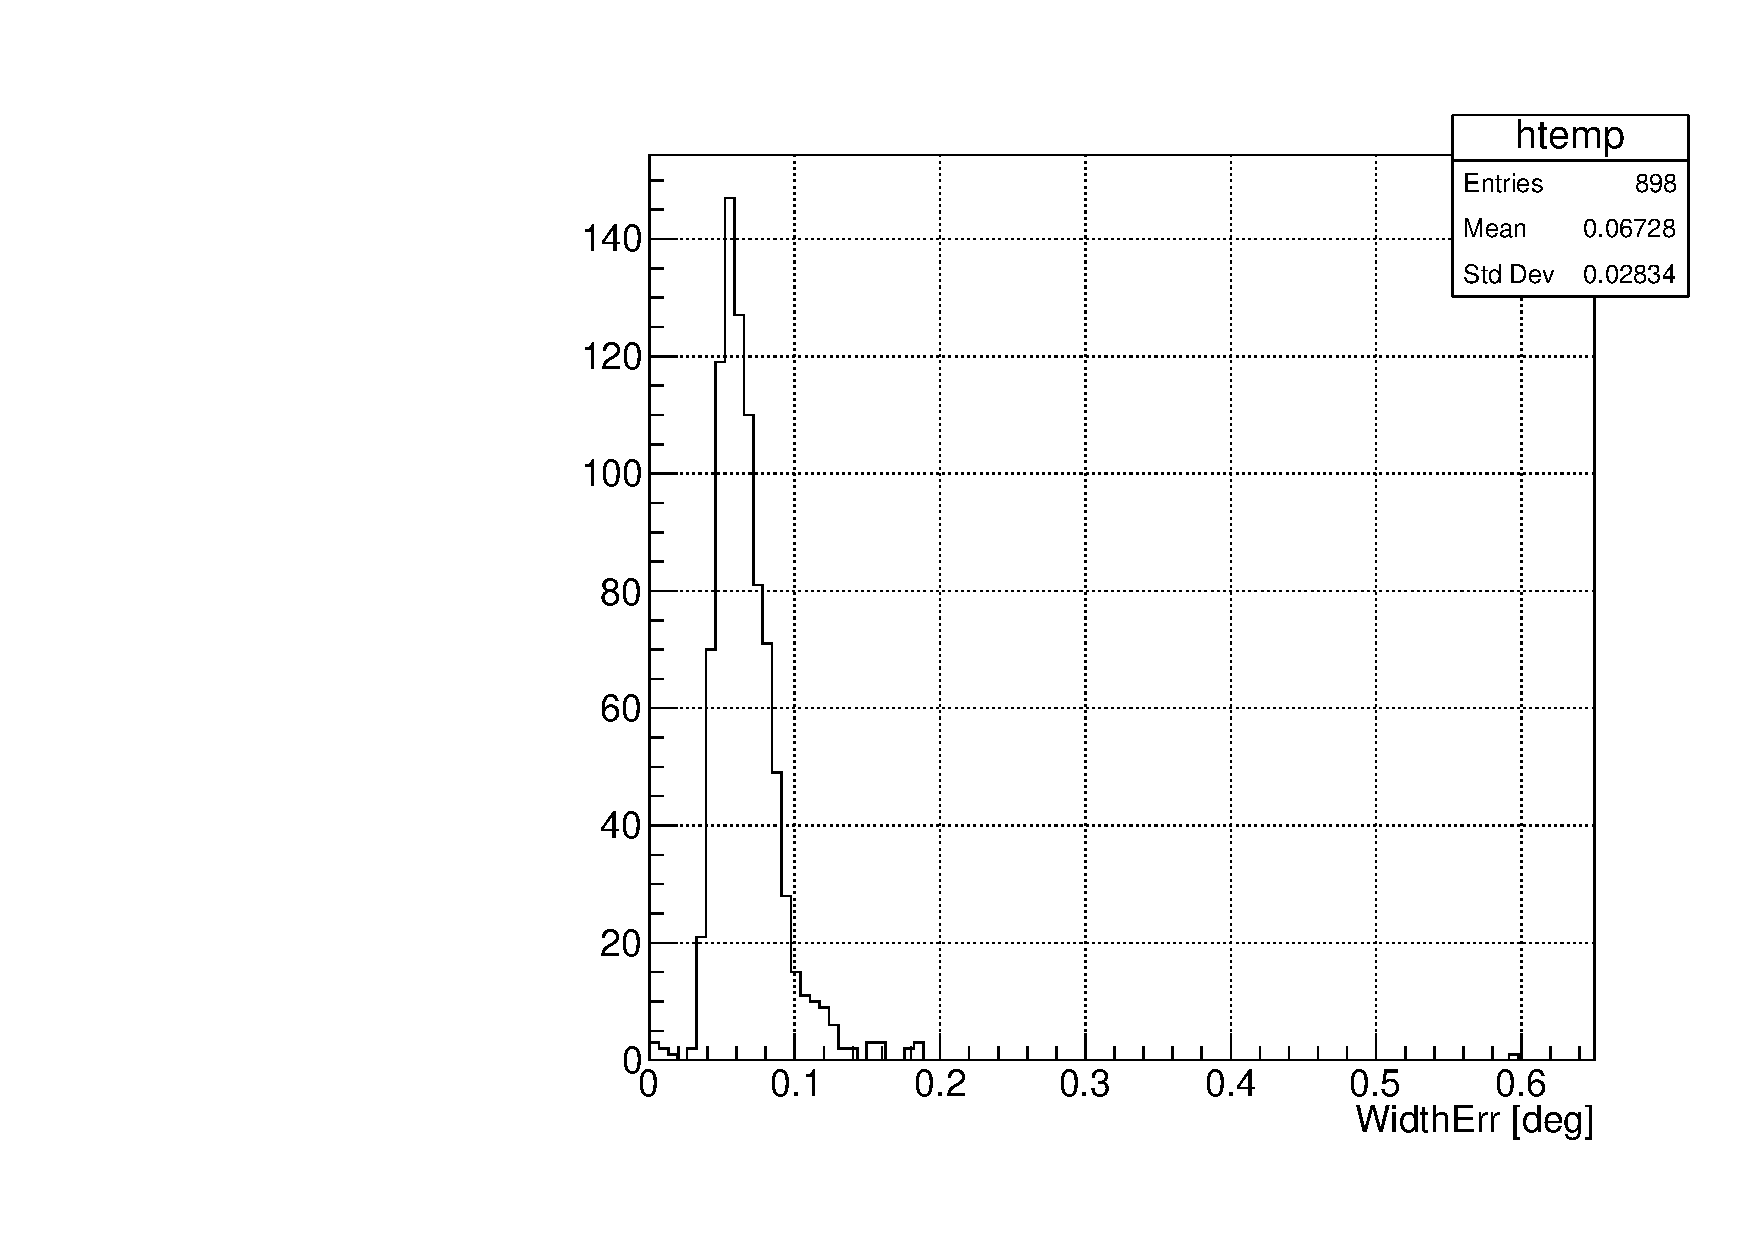
\includegraphics[width=.4\linewidth]{plots/2018/PhiWidthErr.pdf}\\
    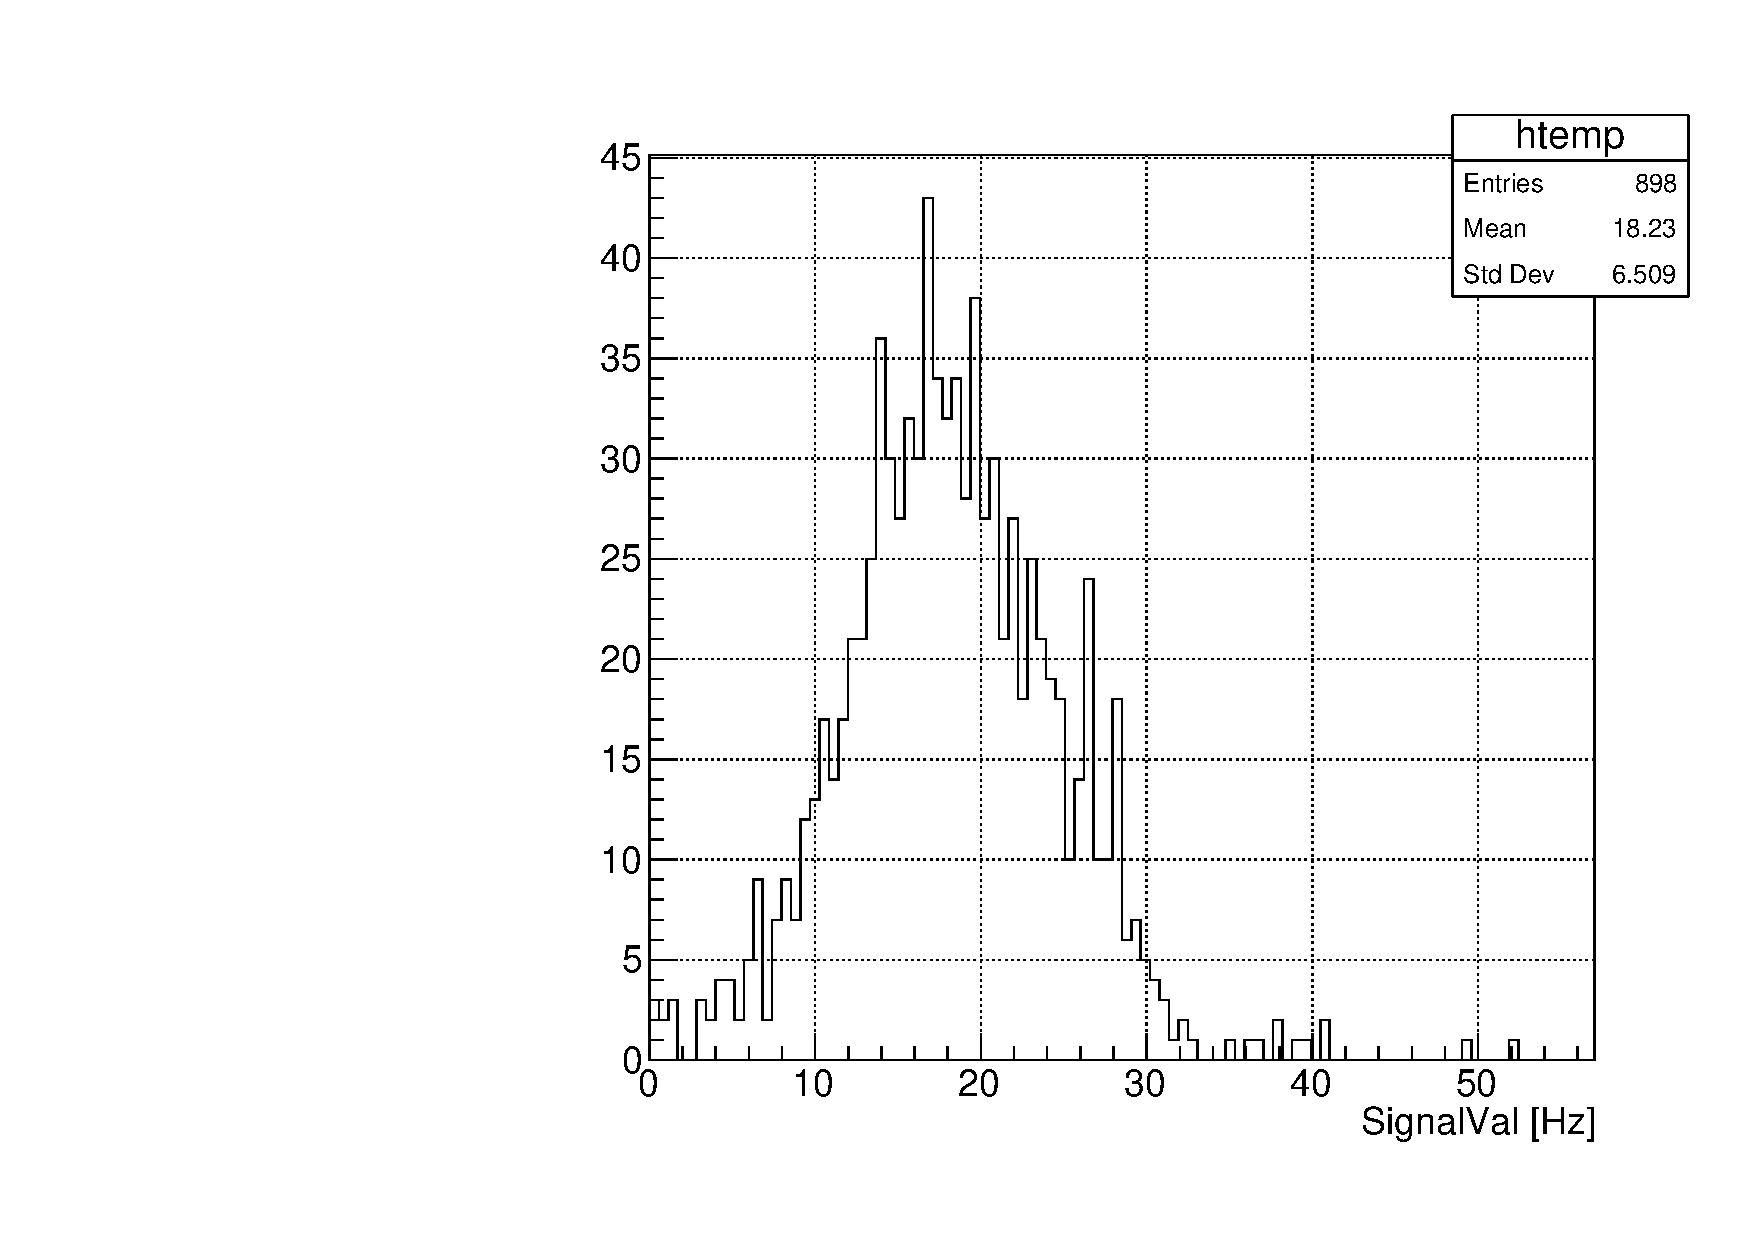
\includegraphics[width=.4\linewidth]{plots/2018/PhiSignalVal.pdf}
    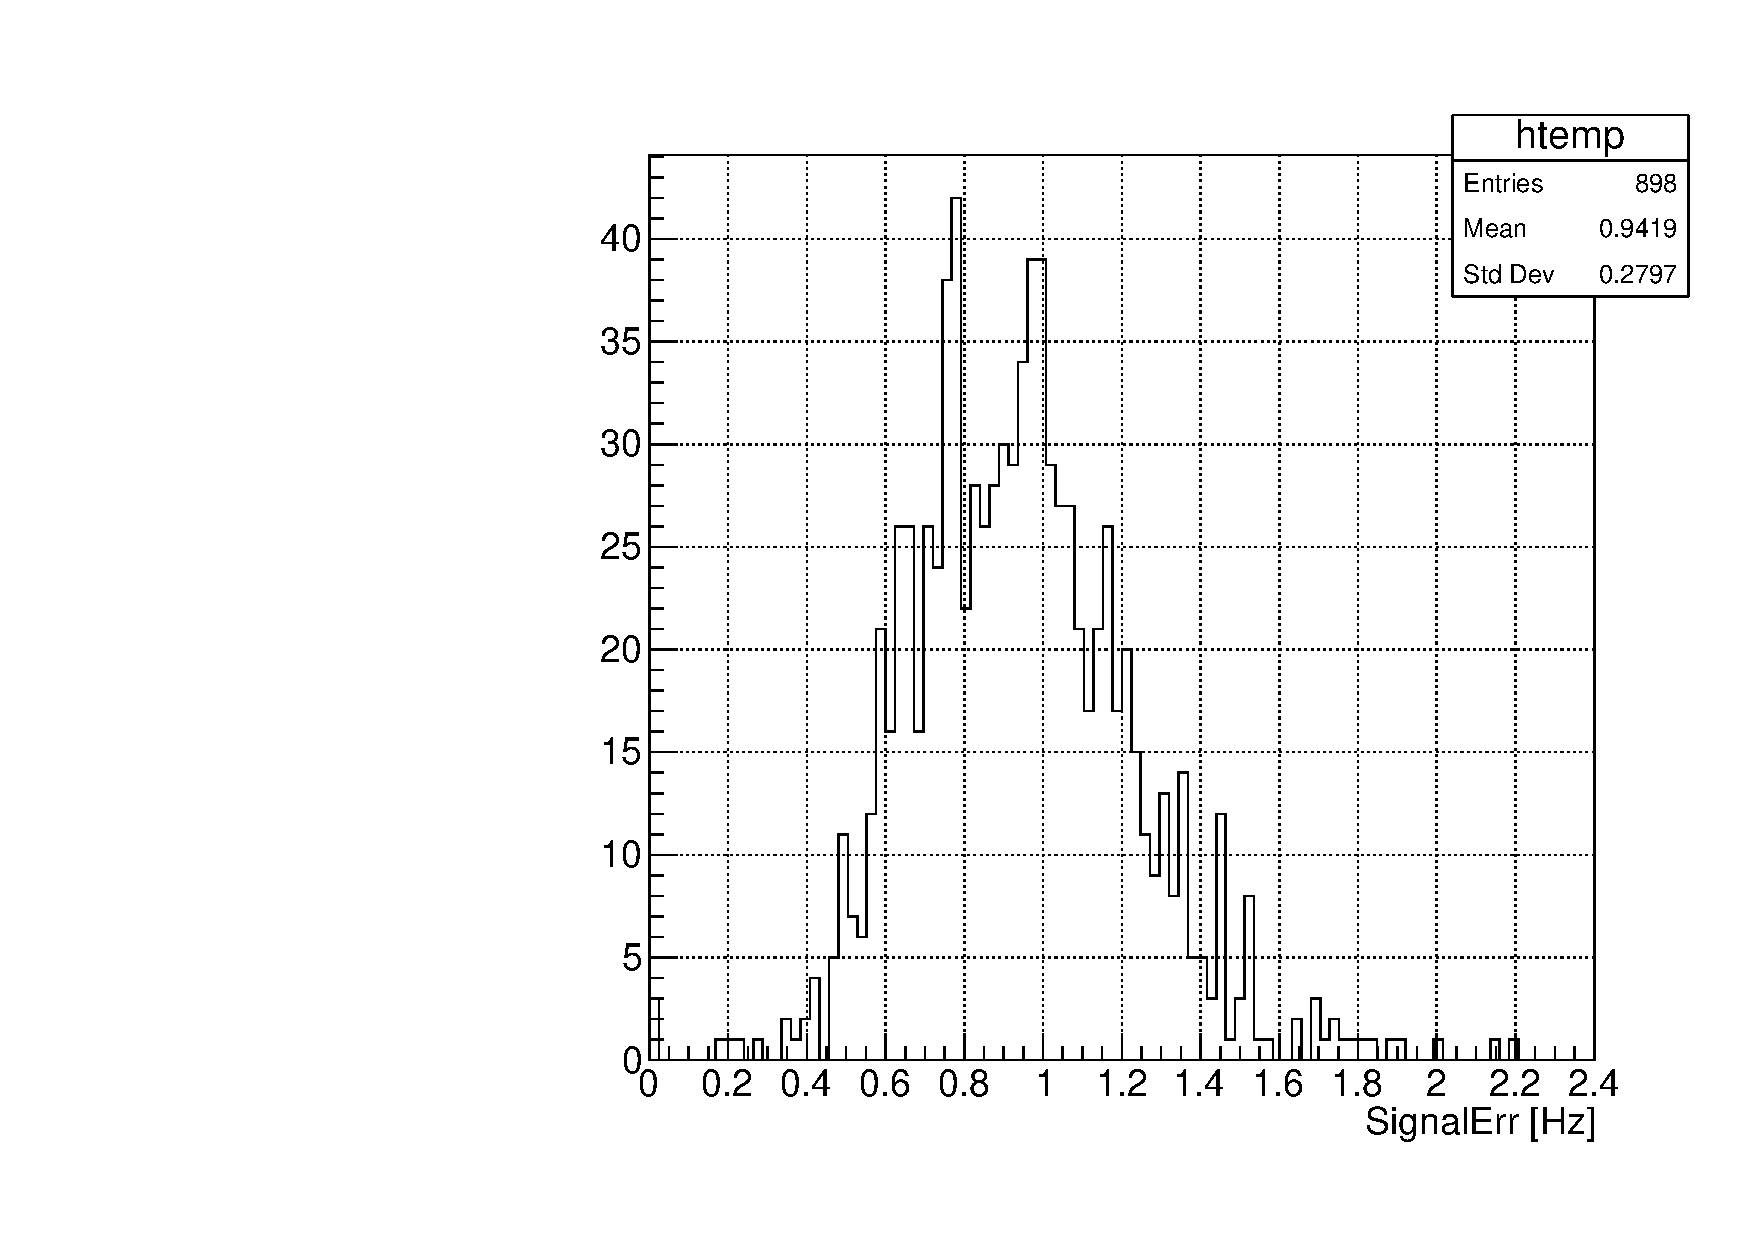
\includegraphics[width=.4\linewidth]{plots/2018/PhiSignalErr.pdf}\\
    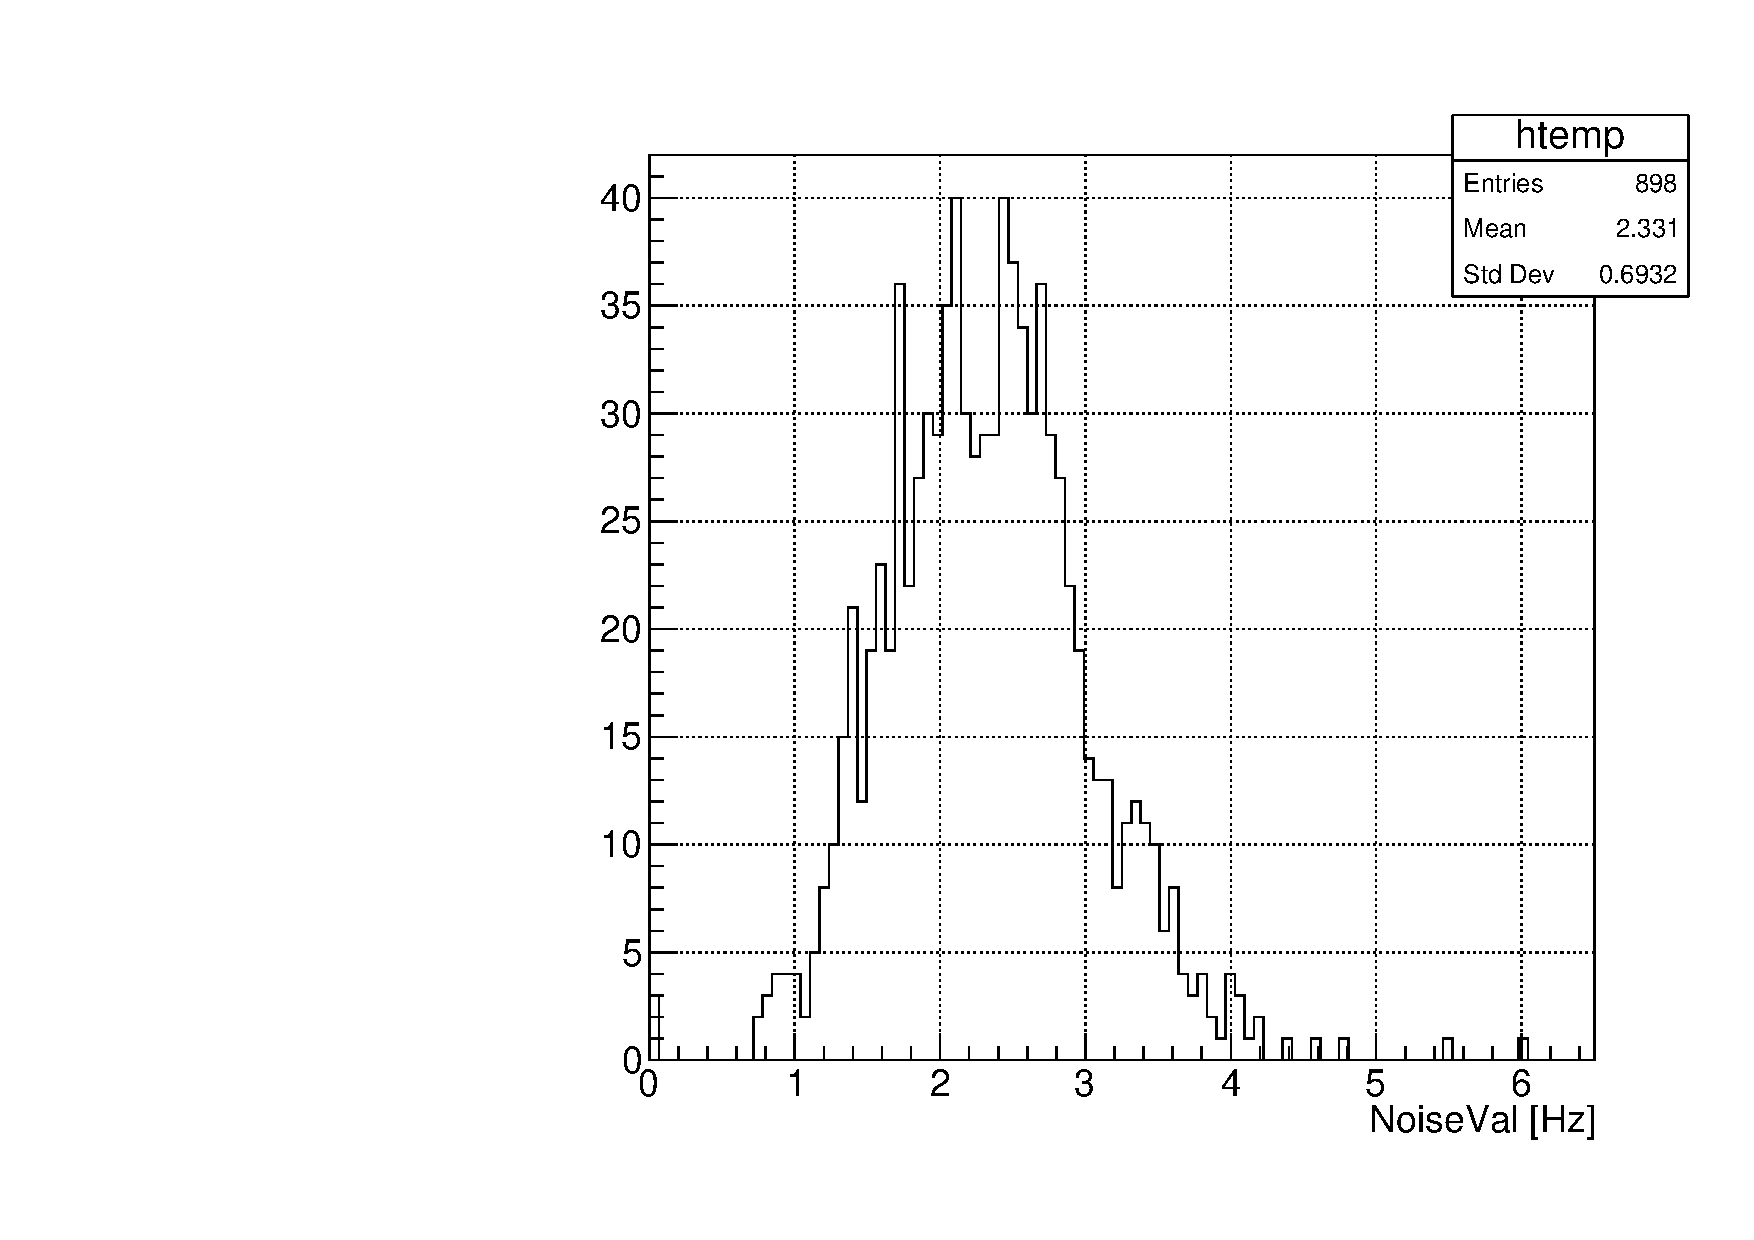
\includegraphics[width=.4\linewidth]{plots/2018/PhiNoiseVal.pdf}
    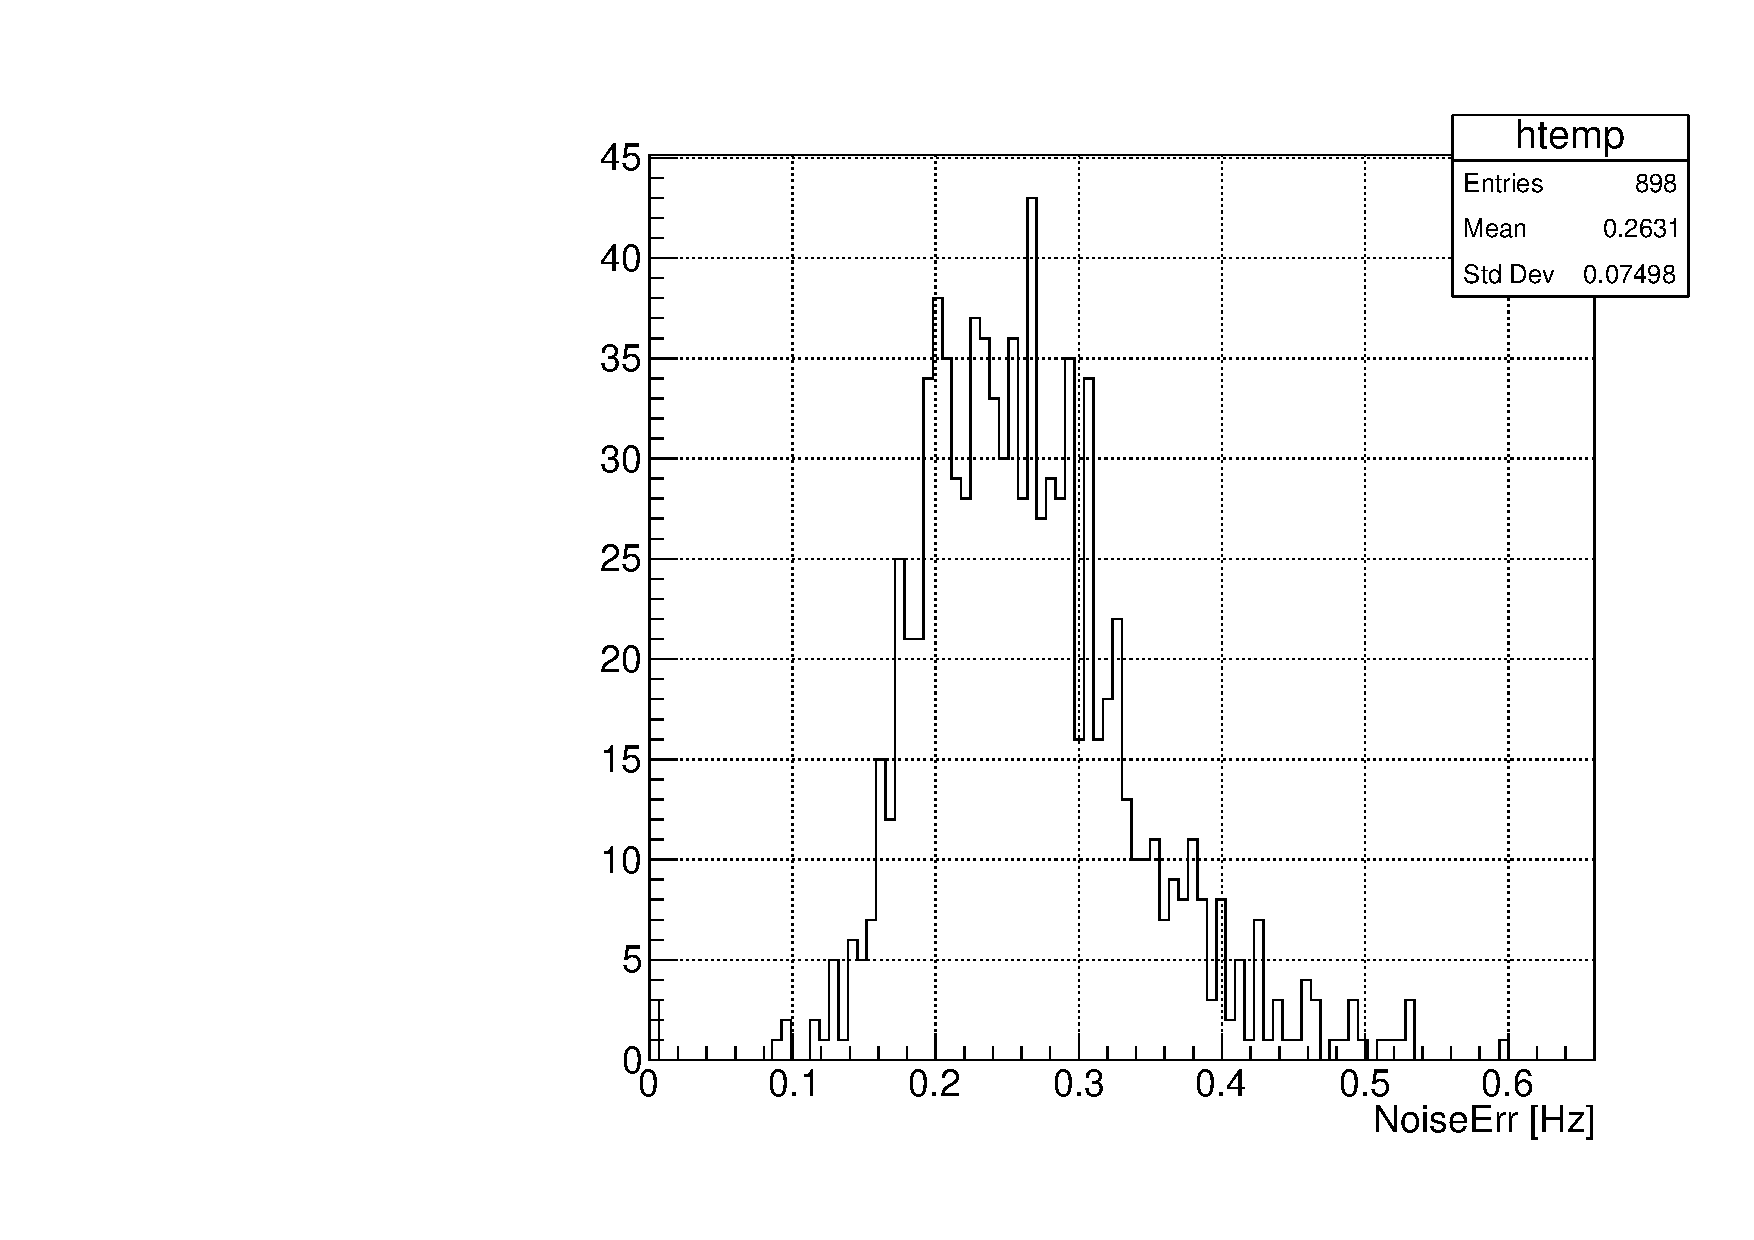
\includegraphics[width=.4\linewidth]{plots/2018/PhiNoiseErr.pdf}
    \caption{Fitted parameter values (left) and errors (right) for $\phi$ position fits.}
    \label{fig:zfitpars}
\end{figure}
